\documentclass[11pt]{article}
\usepackage[sc]{mathpazo} %Like Palatino with extensive math support
\usepackage{fullpage}
\usepackage[authoryear,round,sectionbib,sort]{natbib}   % omit 'round' option if you prefer square brackets
\let\cite\citep


\linespread{1.7}
\usepackage[utf8]{inputenc}
\usepackage{lineno}
\usepackage{titlesec}

\usepackage{graphicx,float}
% for setting up equations
\usepackage{amsmath}

\titleformat{\section}[block]{\Large\bfseries\filcenter}{\thesection}{1em}{}
\titleformat{\subsection}[block]{\Large\itshape\filcenter}{\thesubsection}{1em}{}
\titleformat{\subsubsection}[block]{\large\itshape}{\thesubsubsection}{1em}{}
\titleformat{\paragraph}[runin]{\itshape}{\theparagraph}{1em}{}[. ]\renewcommand{\refname}{Literature Cited}



\usepackage{xcolor}
\newcommand{\tom}[2]{{\color{red}{#1}}\footnote{\textit{\color{red}{#2}}}}

%%%%%%%%%%%%%%%%%%%%%
% Line numbering
%%%%%%%%%%%%%%%%%%%%%
%
% Please use line numbering with your initial submission and
% subsequent revisions. After acceptance, please turn line numbering
% off by adding percent signs to the lines %\usepackage{lineno} and
% to %\linenumbers{} and %\modulolinenumbers[3] below.
%
% To avoid line numbering being thrown off around math environments,
% the math environments have to be wrapped using
% \begin{linenomath*} and \end{linenomath*}
%
% (Thanks to Vlastimil Krivan for pointing this out to us!)

\title{Increasing prevalence of plant-fungal symbiosis over two centuries of climate change}

% This version of the LaTeX template was last updated on
% September 28, 2022.

%%%%%%%%%%%%%%%%%%%%%
% Authorship
%%%%%%%%%%%%%%%%%%%%%
% Please remove authorship information while your paper is under review,
% unless you wish to waive your anonymity under double-blind review. You
% will need to add this information back in to your final files after
% acceptance.

\author{Joshua C. Fowler$^{1,\ast}$ \\
	Tom E. X. Miller$^{1}$}
\date{}

\begin{document}
	
	\maketitle
	
	\noindent{} 1. Rice University, Department of BioSciences, Houston, Texas 77006;


	\noindent{} $\ast$ Corresponding author; e-mail: jcf3@rice.edu.
	
	\bigskip
	
	\textit{Manuscript elements}: Figure~1, figure~2, table~1, appendix~A (for print; including figure~A1, figure~A2, and table~A1), supplemental PDF. Figure~2 is to print in color.
	
	\bigskip
	
	\textit{Keywords}: .
	
	\bigskip
	
	\textit{Manuscript type}: Article. %Or note, natural history miscellany note, comment, reply, invited symposium, featured topic, or historical perspective.
	
	\bigskip
	
	\noindent{\footnotesize Prepared using the suggested \LaTeX{} template for \textit{Am.\ Nat.}}
	
	%\linenumbers{}
	%\modulolinenumbers[3]
	
	\newpage{}
	
	\section*{Abstract}
Many species' distributions and abundances have shifted in response to climate change. 
Most species harbor microbial symbionts that have the potential to influence these responses.
Mutualistic microbial symbionts may provide resilience to environmental change by protecting their hosts from increasing stress. Alternatively, environmental change that causes declines in host or symbiont may disrupt the interaction. 
Microbes can be preserved within the dried plant tissue of herbarium specimens presenting an opportunity to quantify changes across broad temporal and spatial scales. 
We ask how the prevalence of a symbiont of grasses, \emph{Epichloë} fungal endophytes, which can protect hosts from drought, has changed over time in response to climate change, and how these changes vary across the hosts' ranges.
Specifically, we took seed samples from herbarium specimens of three grass host species collected over the last two centuries, quantified fungal hyphae presence within the seeds using microscopy, and evaluated spatial and temporal trends. 
Overall, endophytes have increased in prevalence over the last two centuries from 25\% prevalence to 75\% prevalence on average across the three hosts.
We also found that that the changes in prevalence were associated with observed changes in annual and seasonal climate drivers corresponding with each hosts' peak growing season. 
Thus we provide novel evidence for a cryptic biological response to climate change that may contribute to the resilience of the symbiosis.
	
	\newpage{}
	
	\section*{Introduction}
	
	% The journal does not have numbered sections in the main portion of
	% articles. Please refrain from using section references (à la
	% section~\ref{section:CountingOwlEggs}), and refer to sections by name
	% (e.g. section ``Counting Owl Eggs'').
	
Understanding how biotic interactions are altered by global climate change is a major goal of basic ecological research and conservation management \cite{gilman2010framework,blois2013climate}.
Documented responses to environmental change, such as shifts in species' distributions \cite{aitken2008adaptation} and phenology \cite{piao2019plant}, are typically blind to concurrent changes in associated biotic interactions.
Empirically evaluating these biotic changes, whether interacting species shift in tandem with their partners or not \cite{hillerislambers2013will}, is crucial to predicting future climate change responses. 
Such evaluations have been limited because data on species interactions are limited, with few datasets extending over the long time scales of contemporary climate change \cite{poisot2021global}.


Natural history collections, which were originally collected to study and preserve taxonomic diversity, present a unique opportunity to explore long-term changes in ecological interactions across broad spatial scales \citep{meineke2018unrealized}. 
Natural history collections, built and maintained by the efforts of thousands of scientists, are invaluable time machines, primarily comprised of physical specimens of organisms  along with information about the time and place of their collection. 
These specimens are samples preserving physical legacies of ecological processes and species' interactions from dynamically changing environments across time and space.
Researchers have used plant collections to document climate change responses, including shifts in phenology \citep{willis2017old, park2019herbarium,  berg2019examination}, as well as in rates of pollination \citep{pauw2011reconstruction, duan2019century}, and herbivory \citep{meineke2019herbarium}. 
However, focus has been lacking on long-term changes in a particularly common type of biotic interaction, microbial symbioses.

Microbial symbionts are common to all macroscopic organisms and can have important effects on their hosts' survival, growth and reproduction \cite{rodriguez2009fungal,mcfall2013animals}.
Many microbial symbionts act as mutualists, engaging in reciprocally beneficial interactions with their hosts that ameliorate environmental stress. 
For example, bacterial symbionts of insects, such as \emph{Wolbachia}, can improve their hosts' thermal tolerance \citep{truitt2019wolbachia, renoz2019evolutionary}, and arbuscular mycorrhizal fungi, documented in 70-90\% of families of land plants \citep{parniske2008arbuscular}, allow their hosts to persist through drought conditions by improving water and nutrient uptake \citep{cheng2021elucidating}.
On the other hand, changes in the mean and variance of environmental conditions may disrupt microbial  mutualisms by changing the costs and benefits of the interaction for each partner, leading the interaction to deteriorate \citep{aslan2013mutualism}. 
Coral bleaching (the loss of symbiotic algae) due to temperature stress \citep{sully2019global} is perhaps the best known example, but this phenomenon is not unique to corals.
Lichens exposed to elevated temperatures experienced loss of photosynthetic function along with changes in the community composition of their algal symbionts \citep{meyer2022climate}.
How commonly and under what conditions microbial mutualisms deteriorate or strengthen under climate change remain unanswered questions, but previous work suggests that these alternative responses may depend on the intimacy and specialization of the interaction as well as the physiological tolerances of the mutualists \citep{toby2010mutualisms, warren2014mutualism, rafferty2015phenological}. 

Understanding of how microbial symbioses are affected by climate change is additionally complicated by spatial hetereogeneity in the direction and magnitude of environmental change \cite{ipcc_2021}. 
Beneficial symbionts are likely able to shield their hosts from environmental stress in locations that experience a small degree of change, but symbionts in locations that experience changes of large magnitude may be pushed beyond their physiological limits \cite{webster2008temperature}.
Additionally, symbionts are often unevenly distributed across their hosts' distribution.
Facultative symbionts may be absent from portions of the host range \cite{afkhami2014mutualist}, and hosts may engage with a diversity of partners (different species, or different locally-adapted strains of one species) across their environments \cite{frade2008variation, rolshausen2018quantifying}.
Identifying broader spatial trends in symbiont prevalence is therefore an important step in developing predictions of where to expect changes in the symbiosis in future climates.


\emph{Epichloë} fungal endophytes are specialized symbionts of cool-season grasses, which have been documented in $\sim 30$\% of cool-season grasses \citep{leuchtmann1992systematics}
They are transmitted vertically from maternal plants to offspring through the grasses' seeds.
Vertical transmission creates a feedback between the fitness of host and symbiont \citep{fine1975vectors, douglas1998host, rudgers2009fungus}. 
Over time, endophytes that act as mutualists for their hosts should rise in prevalence within a population. 
\emph{Epichloë} are known to improve their hosts' drought tolerance \cite{decunta2021systematic}, and protect their hosts against herbivores \cite{crawford2010fungal} and pathogens \cite{xia2018role} likely through the production of a diverse suite of alkaloids and other secondary metabolites.
The fitness feedback induced by vertical transmission leads to the prediction that endophyte prevalence should be high in populations where these fitness benefits are most important. 
Previous survey studies have documented large-scale spatial patterns in  endophyte prevalence structured by environmental gradients \citep{granath2007variation,bazely2007broad, afkhami2012fungal,sneck2017variation}.
We predicted that prevalence should also track temporal changes in environmental drivers that elicit these fitness benefits.
For example, endophyte-mediated drought tolerance should lead prevalence to increase in regions where precipitation declines over time.
Early research on \emph{Epichloë} used herbarium specimens to describe the broad taxonomic diversity of hosts \citep{white1985endophyte}. 
Grasses are commonly identified and collected based on the presence of their reproductive structures meaning that collected specimens typically contain seeds, conveniently preserving the fungi along with their host plants on herbarium sheets. 
This creates the opportunity to leverage the unique spatio-temporal sampling of herbarium collections to examine the response of the symbiosis to historical climate change.

In this study, we assessed for the first time the long-term responses of endophyte symbiosis to climate change through the use of herbarium specimens of three \emph{Epichloë} endophyte host species, \emph{Agrostis hyemalis}, \emph{Agrostis perennans}, and \emph{Elymus virginicus}.
We first address questions describing spatial and temporal trends in endophyte prevalence: (i) How does endophyte prevalence vary across space?, (ii) How has endophyte prevalence changed over time? and (iii) How have temporal changes in endophyte prevalence differed across space?
To answer these questions, we fit a spatio-temporal statistical model of endophyte prevalence.
and evaluated the predictive ability of the model using contemporary endophyte surveys as out-of-sample test data, an important but rarely used strategy in ecological studies \cite{tredennick2021practical}. 
We then address how climate change may be driving these trends in endophyte prevalence by addressing the question: (iv) What is the relationship between variation in temporal trends in endophyte prevalence and changes in climate drivers?
We examined 1,865 specimens collected across across eastern North America between 1824 and 2019.
	
\section*{Methods}
        \subsection*{Focal species}
Our surveys focused on three endophyte hosts, \emph{Agrostis hyemalis}, \emph{Agrostis perennans}, and \emph{Elymus virginicus}. Both \emph{Agrostis} species host \emph{Epichloë amarillans} \cite{craven2001multigene, leuchtmann2014nomenclatural}, while \emph{Elymus virginicus} typically hosts \emph{Epichloë elymi} \cite{clay2002evolutionary}.
These $C_3$ grass species are commonly represented in natural history collections with broad distributions covering much the Eastern United States.
\emph{A. hyemalis} is a small short-lived perennial species that germinates in the spring and typically blooms between March and July (most common collection month: May).
\emph{A. perennans} is of similar stature but is longer lived than \emph{Agrostis hyemalis} and blooms in late Summer and early Autumn (most common collection month: September). 
This species is relatively more sparsely distributed, tending to be found in shadier and more moist habitats while \emph{A. hyemalis} is often found in open and recently disturbed ground. 
Both \emph{Agrostis} species are recorded from throughout the Eastern US, but \emph{A. perennans} has a slighty more northern distribution, whereas \emph{A. hyemalis} is found rarely as far north as Canada and is listed as a rare plant in Minnesota.
\emph{E. virginicus} is a larger and relatively longer-lived  species that is more broadly distributed than the \emph{Agrostis} species. 
It begins flowering as early as March or April but continues throughout the Summer (most common collection month: July).

		\subsection*{Herbarium surveys}
We visited herbaria between 2019 and 2022, including The Botanical Research Institude of Texas (which also houses the Vanderbilt University herbarium and the R. Dale Thomas Plant collection from the University of Louisiana at Monroe), the Louisiana State University Herbarium, the Mercer Botanic Garden Herbarium, Missouri Botanic Garden's Herbarium, the S.M. Tracy Herbarium at Texas A\&M, the University of Kansas Herbarium, the Robert Bebb Herbarium at the University of Oklahoma, the Lundell Herbarium and the UT Herbarium at the University of Texas, and Oklahoma State University Herbarium (See Table A1 for a summary of specimens included from each collection). 
In total, we quantified endophyte symbiosis for $964$ \emph{A. hyemalis} specimens collected between 1824 and 2019, $299$ \emph{A. perennans} specimens collected between 1863 and 2017, and $602$ \emph{E. virginicus} specimens collected between 1839 and 2017 (Fig. 1, Fig 2A).
Our sampling plan was designed to minimize damage to these specimens.
We chose our focal species in part because they are commonly represented in herbarium collections, and produce high numbers of seeds, meaning that small samples would not diminish the value of the specimens for future studies. 
We collected 5-10 seeds per specimen after examining the herbarium sheet under a dissecting microscope to ensure that we collected mature seeds, not florets or unfilled seeds, fit for our purpose of identifying fungal endophytes with microscopy.
We excluded specimens for which information about the collection location and date were unavailable.
Each specimen was assigned geographic coordinates based on collection information recorded on the herbarium sheet using the geocoding functionality of the ggmap R package \citep{kahle2019package}.
Many specimens had digitized collection information readily available, but for those that did not, we transcribed information from pictures of the specimens. 
Collections were geo-referenced to the nearest county centroid, or nearest municipality when that information was available. 
For a few of the oldest specimens, only information at the state level was available, and so we used the state centoid.


After collecting seed samples, we quantified the presence or absence of \emph{Epichloë} fungal hyphae, which grow intercellularly, in each specimen using microscopy. 
We first softened seeds with a 10\% NaOH solution, then stained the seeds with aniline blue dye and squashed them under a microscope cover slip. 
We examined the squashed seeds for the presence of fungal hyphae at 100X magnification \cite{bacon2018stains}.
In some cases, the tissues examined during microscopy came from flowers or otherwise non-viable seeds, which were excluded from the seed counts for that specimen.
On average we scored 4.7 seeds per specimen in \emph{A. hyemalis}, 5 seeds per specimen in \emph{A. perennans}, and 3.8 seeds per specimen in \emph{E. virginicus}.
Due to imperfect vertical transmission \cite{afkhami2008symbiosis}, it is possible that symbiotic host-plants produce a mixture of symbiotic and non-symbiotic seeds. 
We therefore designated each specimen as symbiotic if endophyte hyphae were observed in one or more seeds, or non-symbiotic if hyphae were observed in zero seeds. 
To capture uncertainty in the identification process, we recorded both a "liberal" and a "conservative" endophyte status for each plant.  
When we identified potential endophytes with unusual morphology, low uptake of stain, or a small amount of fungal hyphae across the scored seeds, we recorded a positive liberal status (more likely to be a true endophyte) and a negative conservative status (less likely to be a true endophyte). 
$89$\% of scored plants had matching liberal and conservative endophyte statuses, reflecting high confidence in endophyte identification.
The following analyses presented in the main text used the liberal statuses, but we repeated all analyses with the conservative statuses which yielded qualitatively similar results (Figure A5). 

\begin{figure}[H]
	\centering
	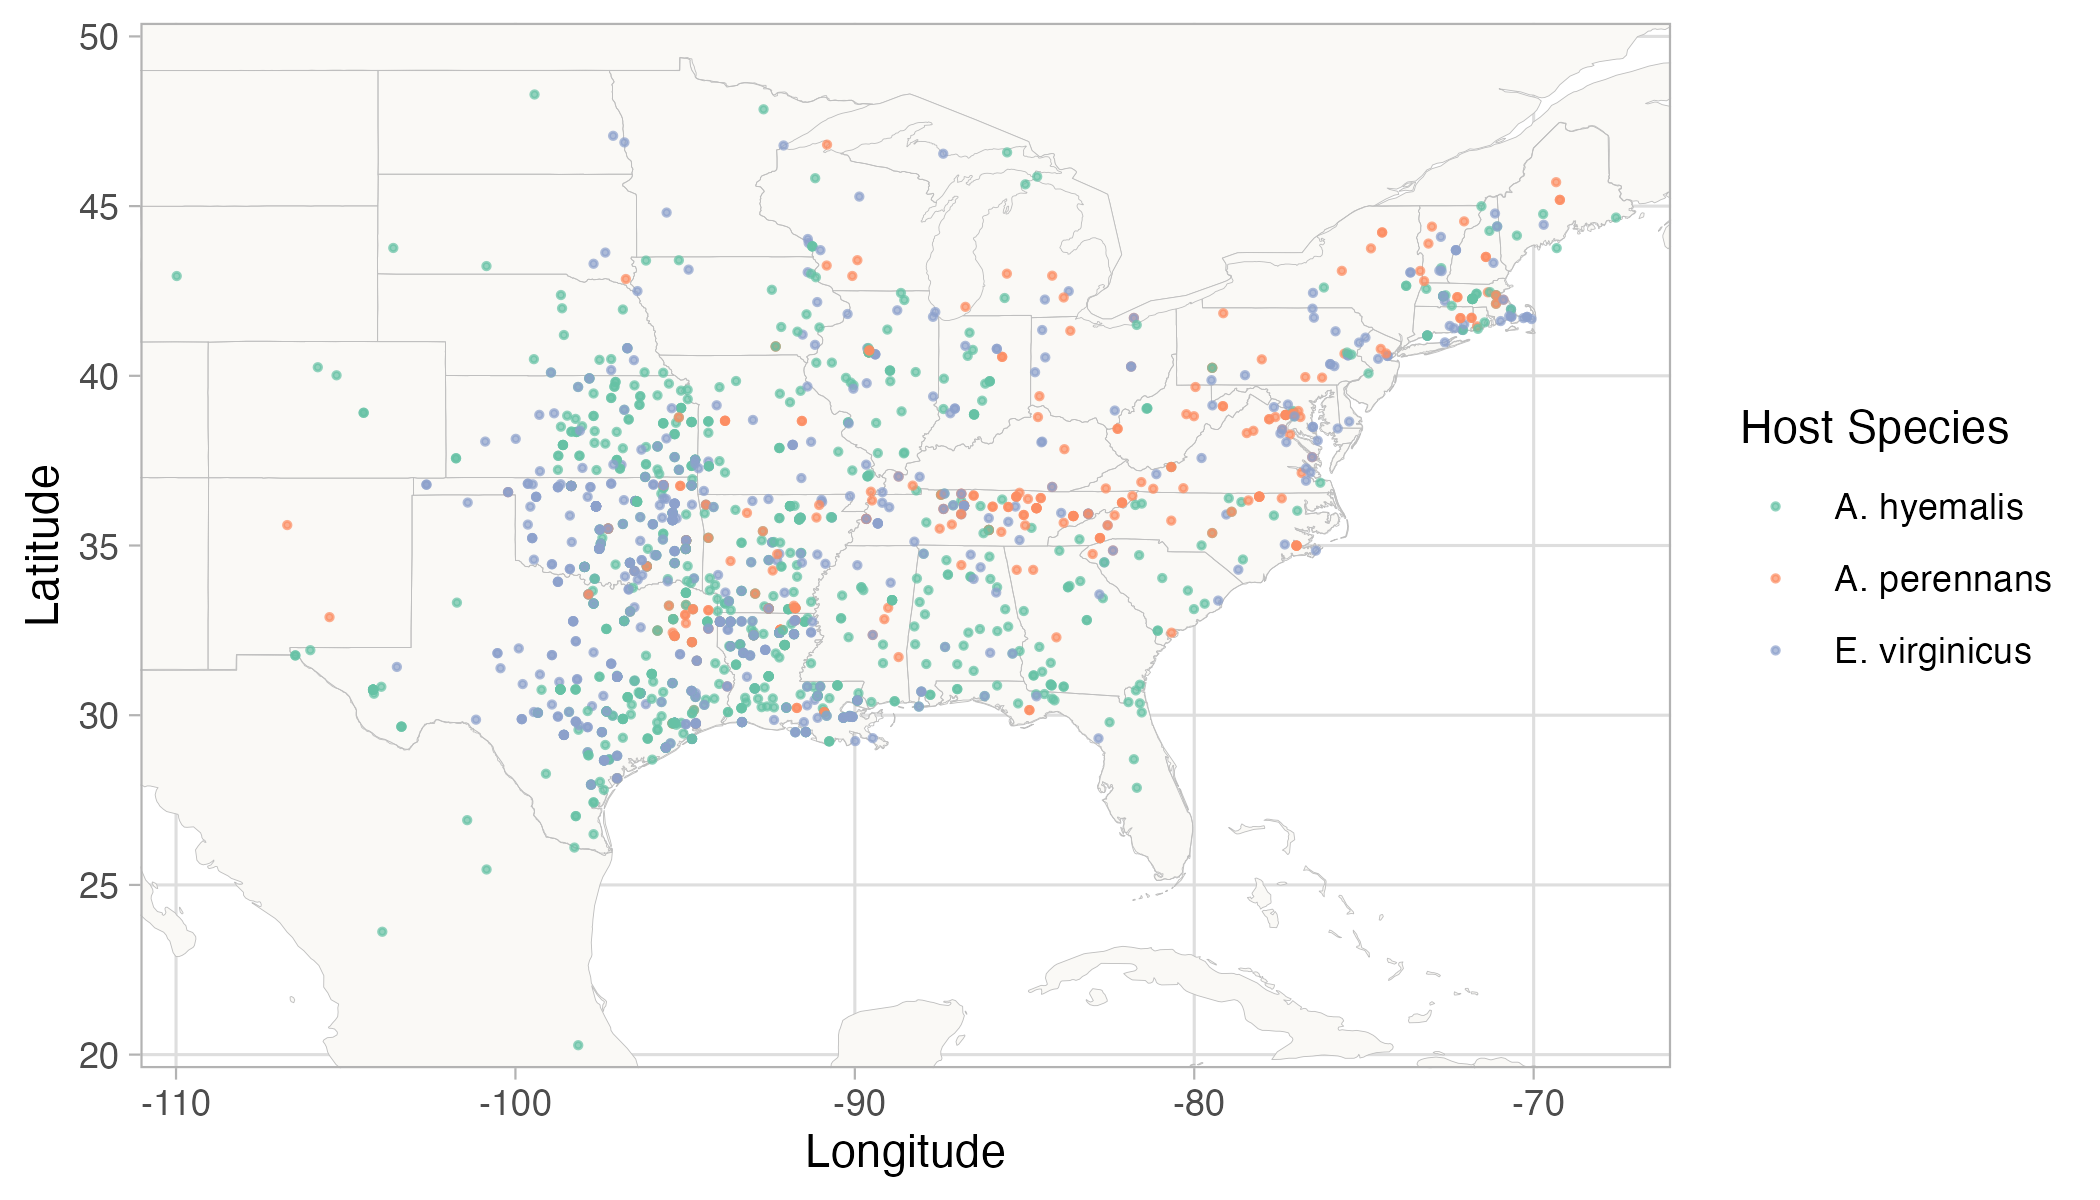
\includegraphics[width = \linewidth]{collections_map.png}
	\caption{\textbf{Collection locations of herbarium specimens sampled for endophyte presence absence}. Color designates host species ( \emph{A. hyemalis} (green), \emph{A. perennans} (orange), \emph{E. virginicus} (purple))}
\end{figure}


\subsection*{Assessing spatial and temporal changes in endophyte prevalence}
To quantify spatial and temporal trends in endophyte prevalence, we used an approximate Bayesian method, Integrated Nested Laplace Approximation (INLA), to fit a spatio-temporal model of endophyte prevalence.
Compared to MCMC Bayesian methods, INLA provides a computationally more efficient method of ascertaining model posteriors for certain models that can be formulated as latent Gausssian Models.  \cite{rue2009approximate}. 
Many common statistical models, including structured and unstructured mixed-effects models, can be represented as latent Gaussian Models. 
Fitting models with structured spatial effects is possible with MCMC sampling but can require long computation times, making INLA an effective alternative, which has been used to model spatial patterns in flowering phenology \cite{willems2022forest}, habitat overlap between marine predators and prey \cite{sadykova2017bayesian}, the distribution of temperate trees \cite{engel2022spatial} as well as the population dynamics of endangered amphibians \cite{knapp2016large} and other ecological processes \cite{beguin2012hierarchical}.

We modeled endophyte presence/absence ($P$) as a Bernoulli response variable for specimen $i$ of host species $h$.

\begin{subequations}
		\label{eq:trends}
		\begin{align}
		P_{i,h} \sim Bernoulli(\hat{P_{i,h}}) \\
			logit(\hat{P}_{h}) = \beta_{0,h} + 
		\beta_{1,h}*year_{i} + \\
		\beta_{2,h}*year_{i} *lat_{i} + 
		\beta_{3,h}*year_{i} *lon_{i} + 
		\beta_{4,h}*year_{i} *lat_{i}*lon_{i} +\\
		\chi + \omega + \phi
		\end{align}
\end{subequations}

The expected endophyte prevalence, $\hat{P}$, was modelled with intercepts specific to each host species ($\beta_{0}$), slopes for changes over time ($\beta_{1}$) as well as the interaction between time and the specimen's latitude and longitude ($\beta_{2}$, $\beta_{3}$, and $\beta_{4}$). 
To quantify spatial patterns in prevalence, we included a spatially-dependent random intercept, $\phi$.
This random spatial effect was modeled as a stochastic partial differential equation (SPDE) that depended on a covariance matrix according to the proximity of each collection location \citep{lindgren2011explicit,bakka2018spatial}. 
The SPDE model allowed us to flexibly estimate endophyte prevalence at locations across the study region, while accounting for potential spatial autocorrelation between data points via the covariance matrix. 
The covariance matrix was approximated using a Matérn covariance function, with each data point assigned a location according to the nodes of a mesh of non-overlapping triangles across our study area (Fig A2).
We accounted for potential biases introduced during the process of collecting specimens as well as in scoring ability by including random effects specific to each collector $\chi$ and to each scorer $\omega$.
Previous work has questioned whether the behavior of historical botanists and uneven sampling may introduce biases into ecological inferences made from historic collections \cite{kozlov2020biases}. 
Prolific collectors who contribute thousands of specimens may be more or less likely to collect certain species, or specimens with certain traits \cite{daru2018widespread}. 
Similarly, the process of scoring seeds for hyphae involved many individual researchers, who may vary in their likelihood of positively identifying fungal hyphae. 
By including a random effect for collectors and for scorers, we can account for the variance across individual researchers that may bias our predictions of changes in endophyte prevalence.
We performed model fitting using the rINLA package, \citep{lindgren2015bayesian}, with vague priors, and compared models with different sizes of mesh, which had little effect on the resulting model estimates.
Posterior modes were stable indicating that numeric convergence was successful.
We assessed model fit with graphical posterior predictive checks (Fig. A3).
The model performed adequately at classifying the historical data, comparing the accuracy of predictions from the model with observed data (AUC = 0.77; Fig. A4). 
\subsection*{Validating the model with an out-of-sample test}
We used data from contemporary surveys of endophyte prevalence  in \emph{A. hyemalis} and \emph{E. virginicus} as test data to evaluate predictions of the model. 
Surveys of \emph{E. virginicus} were conducted in 2013 as described in \citet{sneck2017variation}, and surveys of \emph{A. hyemalis} took place between 2015 and 2020.
Population surveys of \emph{A. hyemalis} were initially designed to cover longitudinal variation in endophyte prevalence towards its range edge, while surveys of \emph{E. virginicus} were designed to cover latitudinal variation along its range edge. 
In total, we visited 43 populations of \emph{A. hyemalis} and 20 populations of \emph{E. virginicus} across the central southeastern US, in Texas and neighboring states (Fig A4).
During surveys, we collected seeds from up to 30 individuals per location  (average number of plants sampled: 22.9).
We quantified the endophyte status of each individual with staining microscopy as described for the herbarium surveys, and calculated the prevalence of endophytes within the population (proportion of symbiotic plants divided by the number of sampled plants).
The contempory survey period (2013-2020) is at the most recent edge of the time period encompassed by the historical observations used for model fitting.
We compared the model's prediction for these locations to the observed population prevalence.

		\subsection*{Assessing the role of climate drivers}
		
We assessed how the magnitude of climate change may have driven changes in endophyte prevalence by assessing correlations between changes in climate and changes in endophyte prevalence predicted from our spatial model at evenly spaced pixels across the study area. 
We first downloaded monthly temperature and precipitation rasters from the PRISM climate group \citep{daly2013prism} covering the time period between 1895 and 2020 using the 'prism' R package \citep{Rprism2015}. 
Prism provides reconstructions of historic climate variables across the United States by spatially-interpolating weather station data \citep{diLuzio2008constructing}. 
We calculated 30-year climate normals for annual and seasonal mean temperature and cumulative precipitation for the recent (1990 to 2020) and historic (1895 to 1925) periods.
We used three four-month seasons within the year (Spring: January, February, March, April; Summer: May; June, July, August; Autumn: September, October, November, December). 
This division of seasons allowed us to quantify differences in climate associated with the two "cool" seasons  that shoulder summer when we expect our focal species to be most biologically active (\emph{A. perennans}: Spring; \emph{E. virginicus}: Spring and Summer; \emph{A. perennans}: Fall). 
In addition to mean climate conditions, environmental variability  in and of itself can influence population dynamics \cite{tuljapurkar_population_1982} and changes in variability are a key prediction of climate change models \cite{stocker2013technical, ipcc_2021}.
So we calculated the coefficient of variation during each period for each annual and seasonal climate driver as the interannual standard deviation divided by the mean across each 30-year period.
We then took the difference between recent and historic periods for the mean and coefficient of variation for each climate driver (Fig. A5).
Because initial analyses indicated a high degree of collinearity between seasonal and annual changes in temperature, we used annual temperature only, along with annual and seasonal precipitation, in the subsequent analysis.
All together, this left us with measurements of change in 10 potential climate drivers: the mean and coefficient of variation of annual temperature, as well as the mean and coefficient of variation of cumulative annual precipitation, cumulative spring precipitation, cumulative summer precipitation, and cumulative autumn precipitation (Fig A8-A9).

We calculated the relative change in endophyte prevalence across the 1925 to 2020, i.e., the difference between predicted prevalence divided by the endophyte prevalence in 1925, because regions varied in their predicted starting prevalence. 
This time period connects the predicted change in prevalence with the endpoints of the available climate record.
We then calculated the Spearman correlation coefficient between the relative change in endophyte prevalence and each climate driver.
Calculating correlations from many pixels across the study region risks articially inflating confidence in our results due to large sample sizes, and so we repeated this calculation using only a random subsample of 100 pixels across the study region.


%We evaluated how predicted changes in endophyte prevalence ($\Delta{P}$) correlated with %changes in seasonal climate at a grid of points across the study area using linear regression.

%\begin{subequations}
	%\label{eq:climate}
	%\begin{align}
		%\Delta{P} \sim Normal(\mu, \sigma)\\
		%\mu = \beta_{0} + \alpha_{1}*\Delta{Precip_{spring}} + %\alpha_{2}*\Delta{Precip_{summer}} + \alpha_{3}*\Delta{Precip_{autumn} }+ \\ %\alpha_{4}*\Delta{Temp_{spring}} + \alpha_{5}*\Delta{Temp_{summer}}  + %\alpha_{6}*\Delta{Temp_{autumn}} 
%	\end{align}
%\end{subequations}

 %The change in prevalence is determined by an intercept $\beta_{0}$ slopes specific to the seasonal %changes in preciptation ($\alpha_{1}$, $\alpha_{2}$, and $\alpha_{3}$) and in mean %temperature ($\alpha_{4}$, $\alpha_{5}$, and $\alpha_{6}$).
 %We fit models for each host species separately with rINLA using default vague priors.
		
\section*{Results}
\subsection*{Temporal and spatial trends}
We quantified temporal and spatial trends in endophyte prevalence while accounting for potential biases introduced by collectors and by individuals who quantified endophyte presence/absence with the use of random effects. We found no evidence that collector biases influenced our results (collector random effects were consistently small; Fig 2A), while the identity of individual scorers did contribute to observed patterns in endophyte prevalence (3 of the 16 scorers were more likely than average to assign positive endophyte status, as indicated by 95\% credible intervals that do not overlap 0) (Fig 2B). Interpretation of the data without accounting for this source of variation would lead to potentially biased interpretations of temporal and spatial trends.

\begin{figure}[H]
	\label{fig:random_fx}
	\centering
	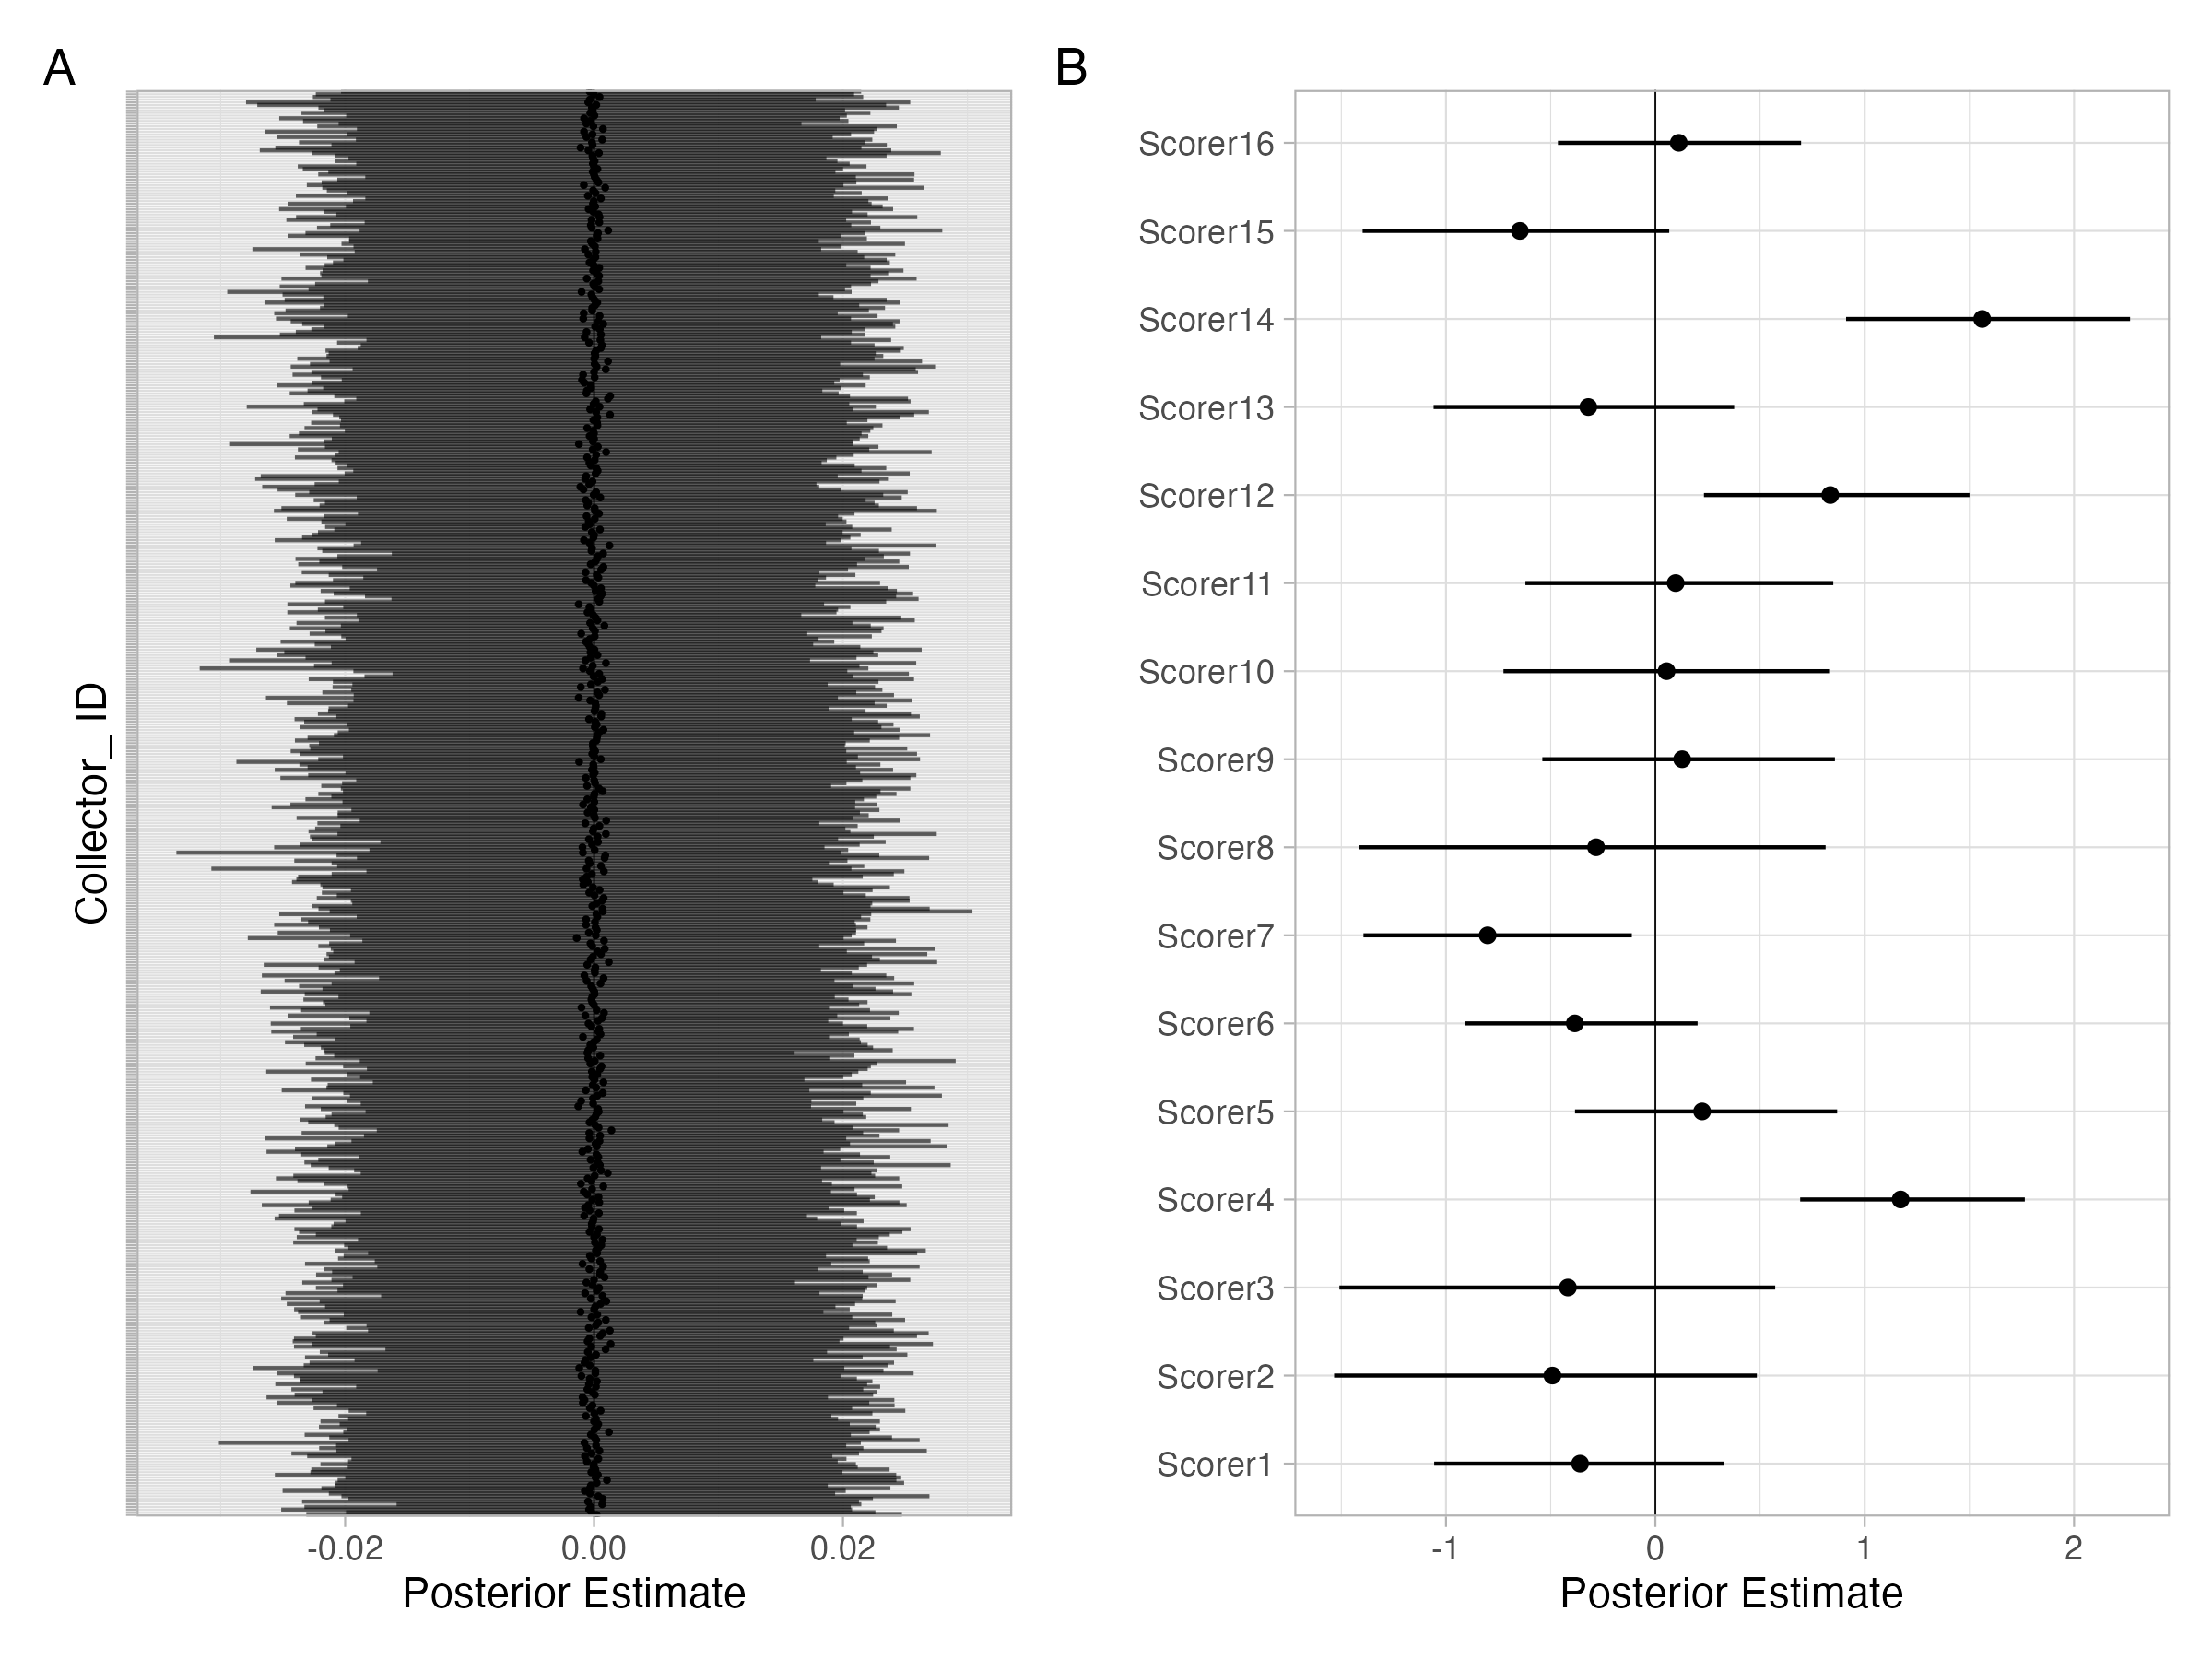
\includegraphics[width = .8\linewidth]{random_fx_plot.png}
	\caption{\textbf{Posterior estimates of (A) collector and (B) scorer random effects.} Points show the posterior mean along with 95\% CI for random effects estimate from 532 collectors and 16 scorers.}
\end{figure}


\subsubsection*{How does endophyte prevalence vary across space?}
Across space, there were clear trends in endophyte prevalence which varied between species (Fig. 3).
We mapped predictions of endophyte prevalence across the area encompassing the sampled herbarium specimens for each species, and area smaller than the full geographic distribution of each species in nature.
\emph{Elymus virginicus} had higher prevalence towards the northern portions of the collection range. 
In contrast, \emph{Agrostis hyemalis} had highest prevalence towards the center of its collection range with regions of low prevalence towards the northeast and towards its western range edge.
\emph{Agrostis perennans} had  highest prevalence towards the westernmost portion of its collection range.
There is considerable uncertainty in the spatial pattern of endophyte prevalence (See Fig. A10 for projections of the 95\% credible interval), however these broad spatial patterns are consistent across the low and high end of model predictions. 

\begin{figure}[H]
	\label{fig:prevalence_map}
	\centering
	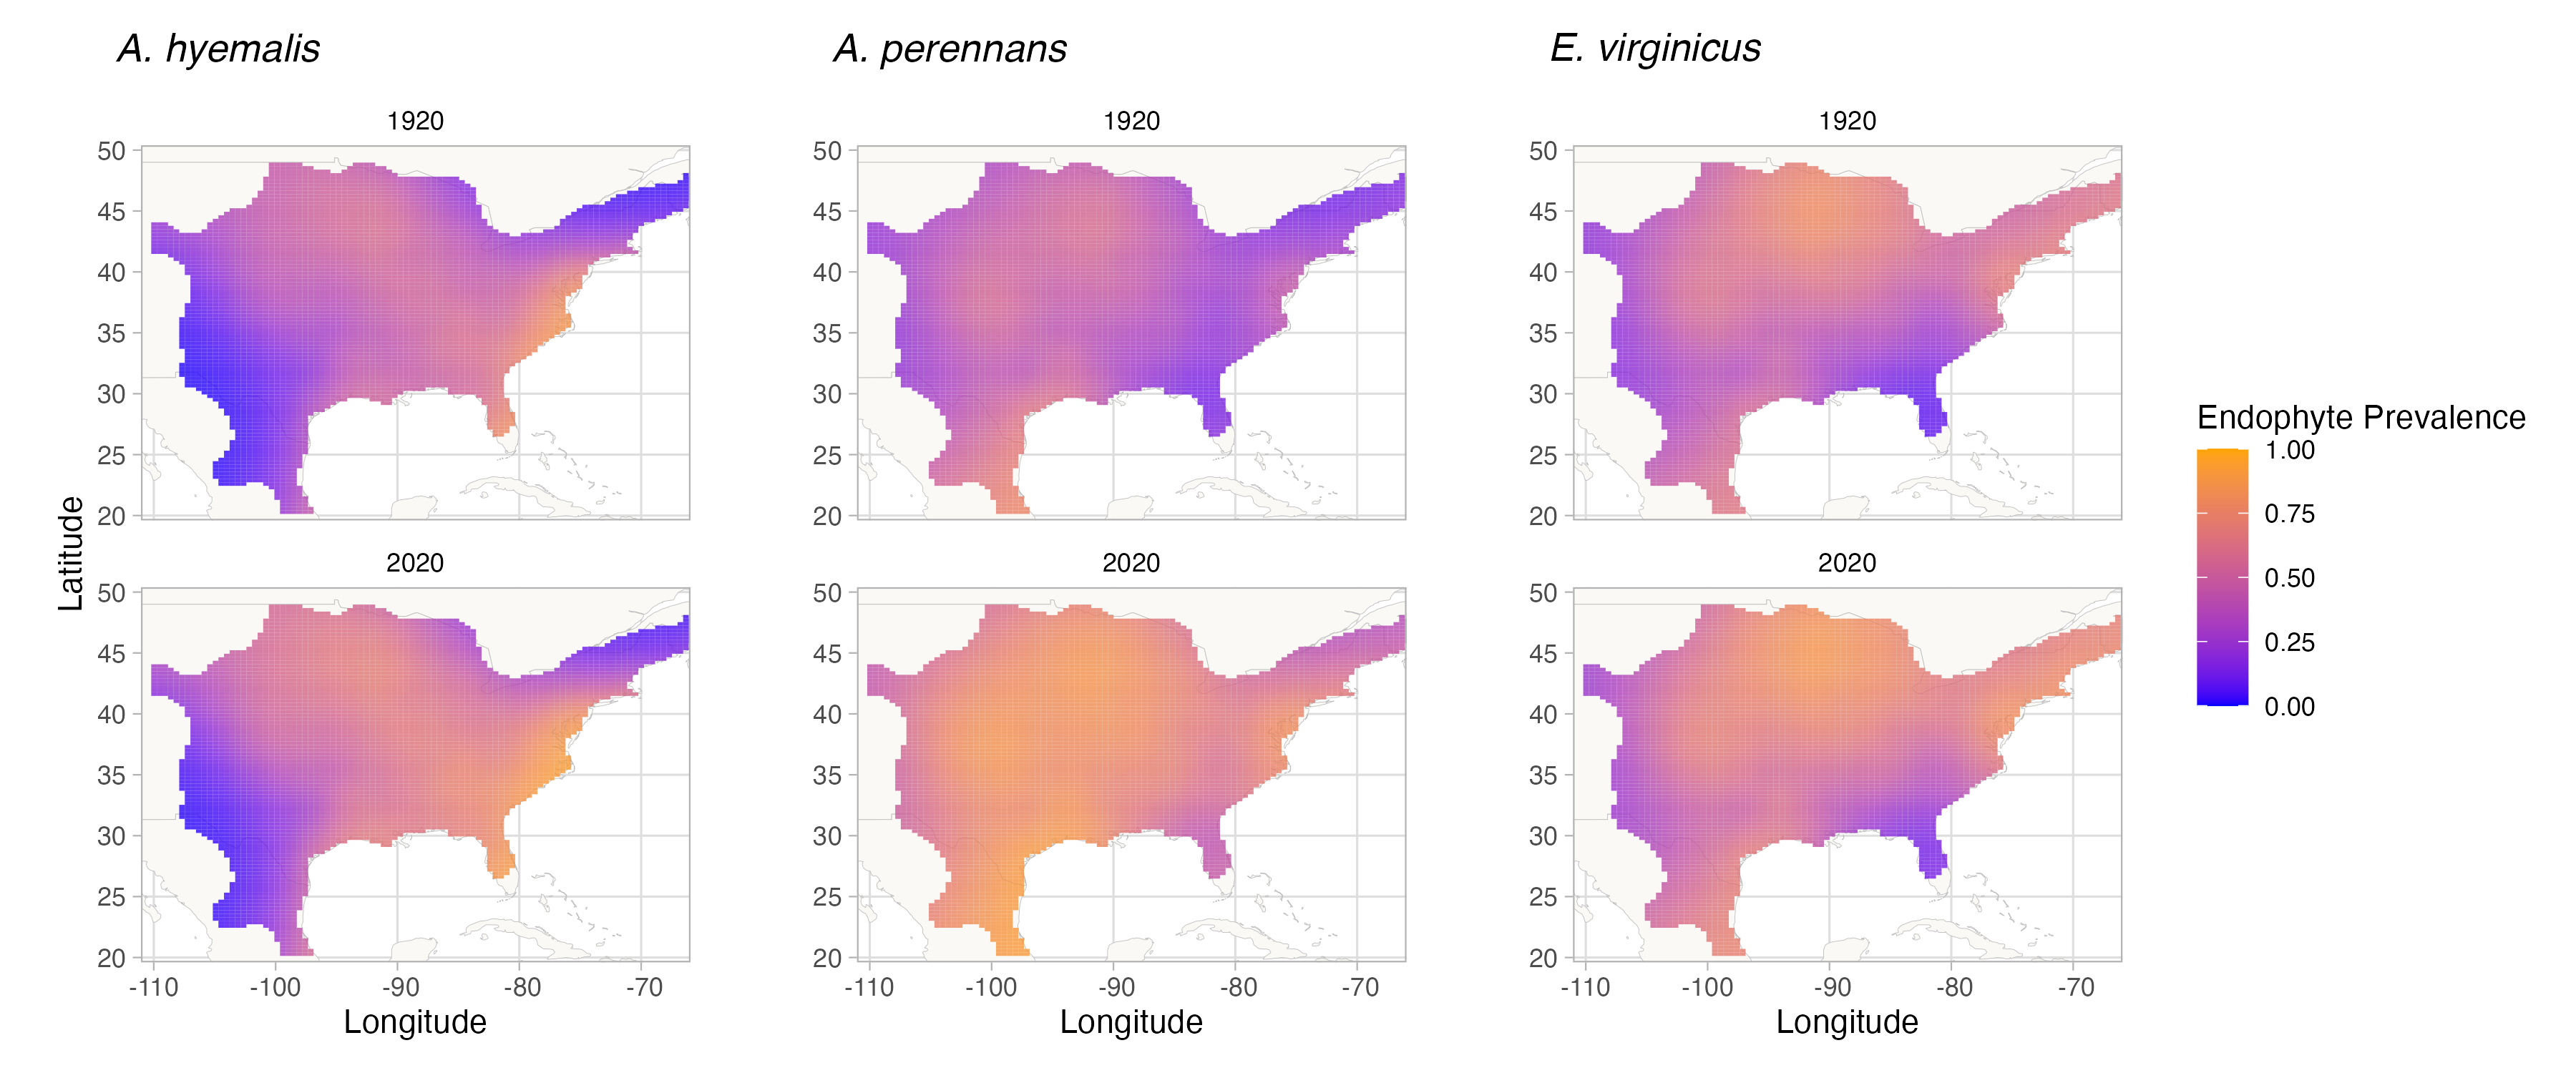
\includegraphics[width = \linewidth]{prevalence_map.png}
	\caption{\textbf{Mean predicted endophyte prevalence for each host species (columns) in 1925 (top row) and 2020 (bottom row)}. Color indicates mean predicted rate of endophyte prevalence across a convex boundary enscribing the collections locations of each species (excluding two disjoint collections of \emph{A. perennans} to the west).}
\end{figure}


\subsubsection*{How has endophyte prevalence changed over time?}
We found that endophyte prevalence increased within the examined specimens over the last two centuries for all three host species (Fig. 4). 
On average, \emph{A. hyemalis} and \emph{E. virginicus} both increased from ~30 \% to over 50\% prevalence across the study region, and \emph{A. perennans} increased from ~ 15\% to over 70\% prevalence.
Rerunning the analysis excluding specimens collected before 1900 when samples are much sparser (Fig. 2A), lead to qualitatively similar predictions, and so we continued analyses with the full dataset. 
Our model indicates a higher certainty that overall temporal trends are positive for \emph{A. hyemalis} and \emph{A. perennans} than for \emph{E. virginicus} (99\% probability of a positive overall year slope in \emph{A. hyemalis}, 89\% probability of a positive overall year slope in \emph{A. perennans}, and 58\% probability of a positive overall year slope in \emph{E. virginicus}) .

\begin{figure}[H]
	\centering
	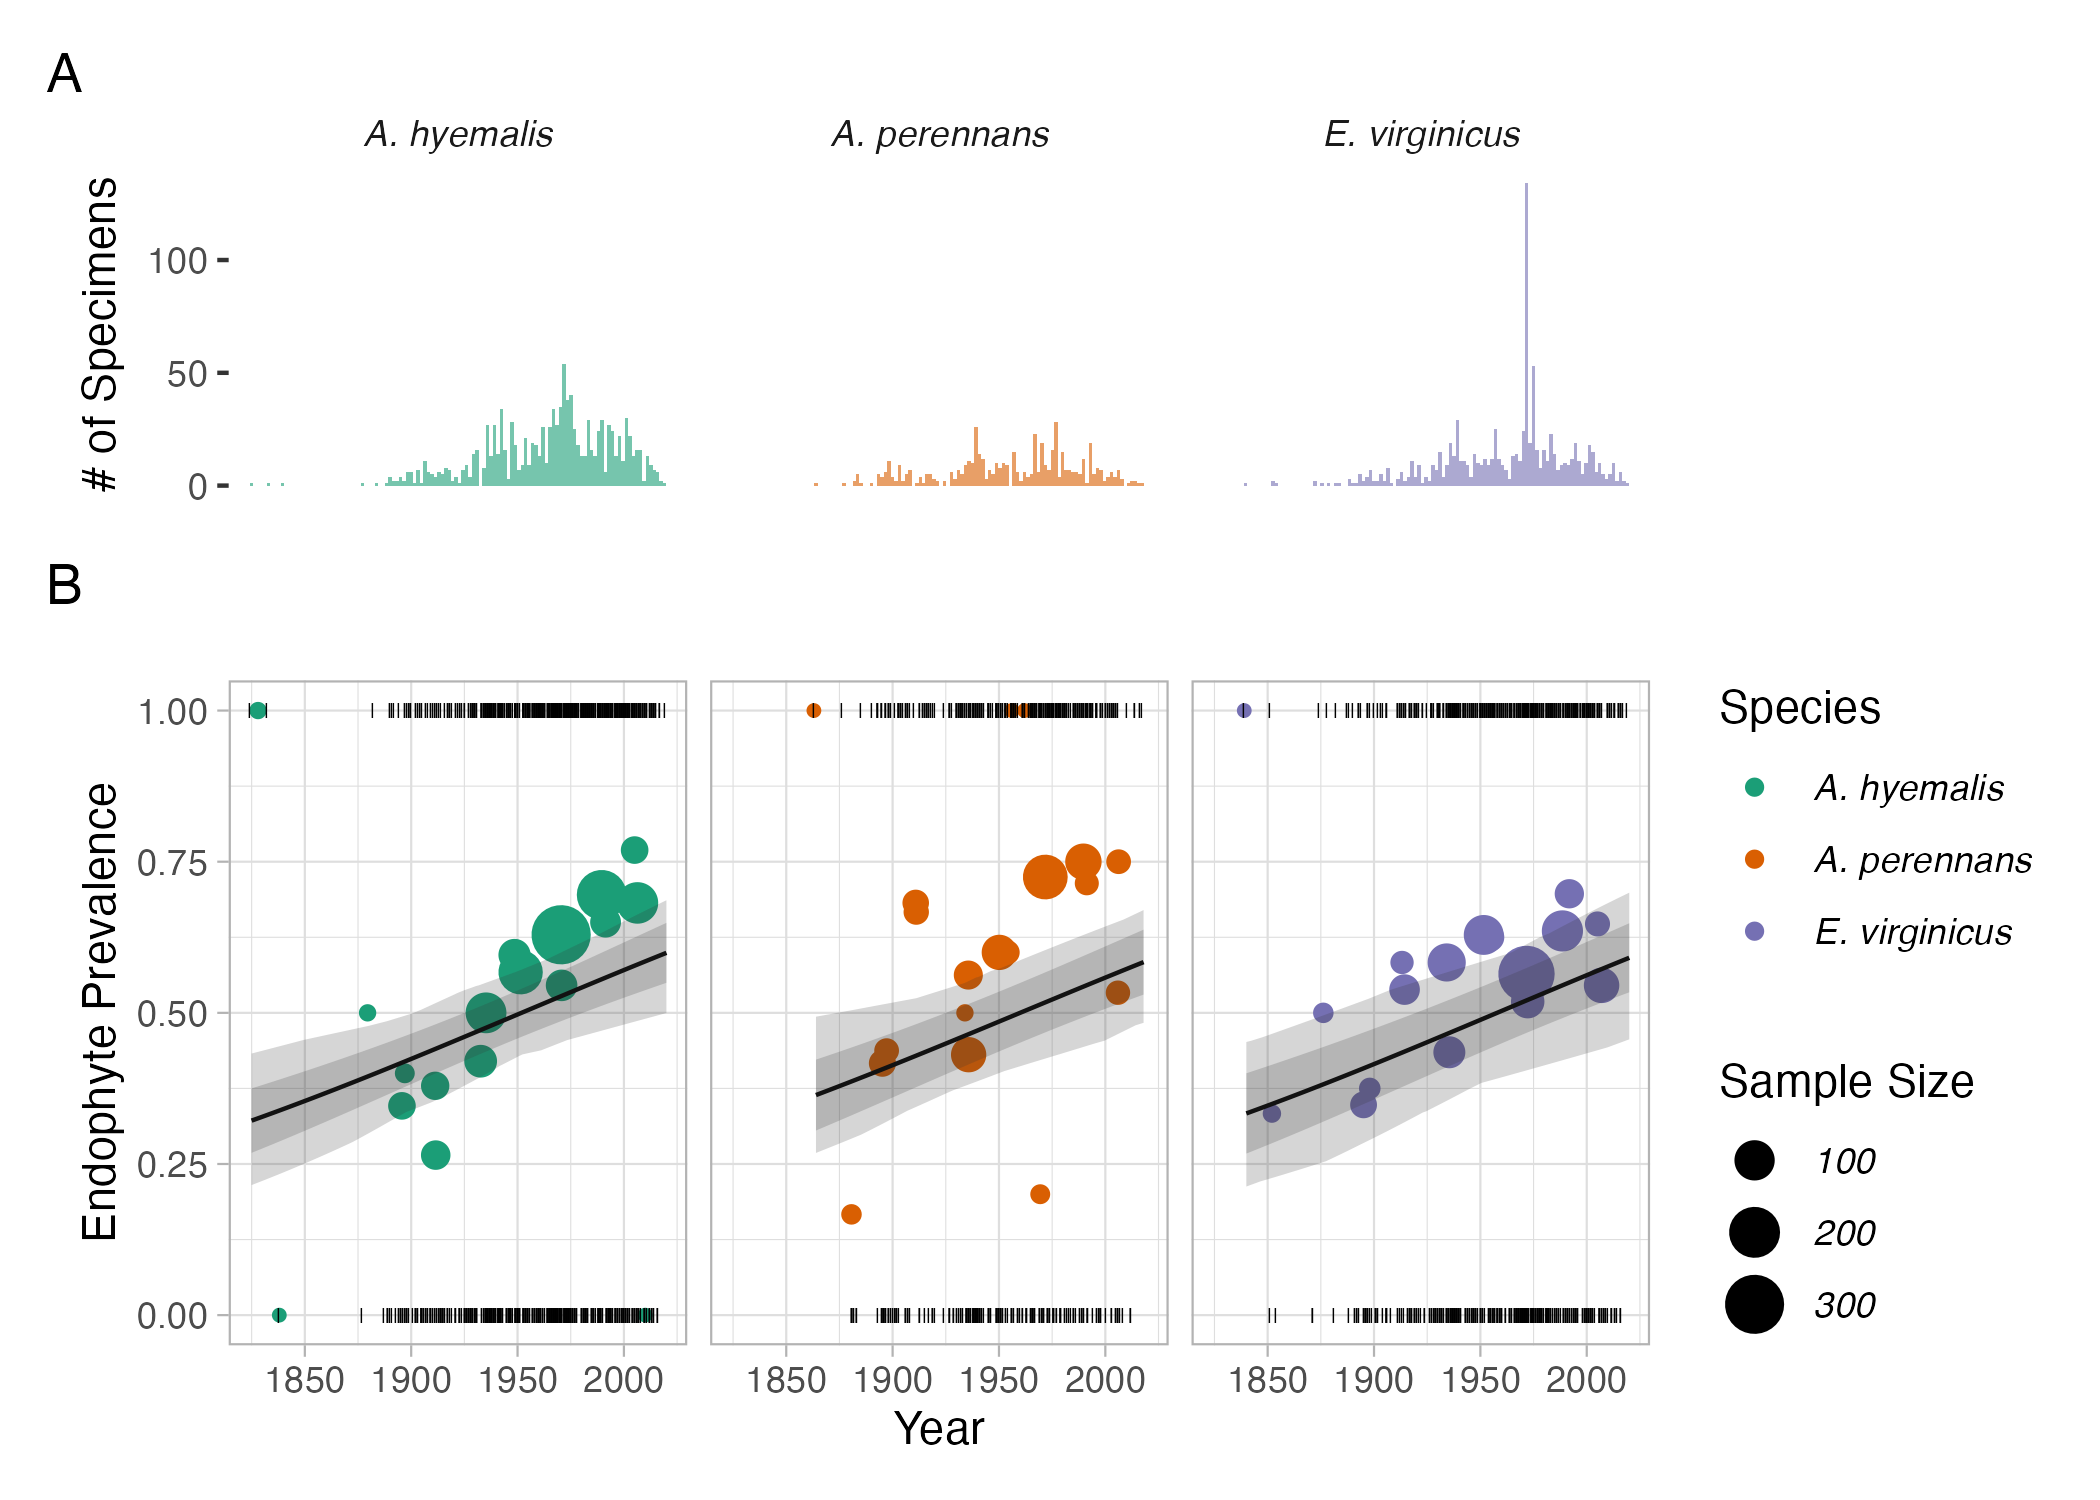
\includegraphics[width = \linewidth]{year_plot.png}
	\caption{\textbf{Temporal trends in endophyte prevalence.} (A) Histograms show the frequency of collection through time for each host species. (B) Colored points are binned means of the observed endophyte presence/absence data (black dashes). Colors represent each host species and point size is determined by the number of specimens. Lines show predicted mean endophyte prevalence over the study period at low (dotted) high (solid) latitudes and along with 95\% CI bands.}
\end{figure}

\subsubsection*{How have temporal changes in endophyte prevalence differed across space?}
Our model revealed that while there was an overall increase in endophyte prevalence, these changes varied across the host species' ranges.
The posterior estimates of the parameters describing space by time interactions, $\beta2$, $\beta3$, and $\beta4$ for each species indicate small effect sizes, but high certainty(i.e, a 99\% posterior probability of a negative interaction between year and latitude for \emph{A. hyemalis}, or a 67\% postterior probabilty of a postitive interaction between year and latitude for \emph{E. virginicus}) (Fig. A5).
In some regions, \emph{A. perennans} experienced increases in percent prevalence by as much as 35 percentage points between 1925 and 2020, while \emph{A. hyemalis} and \emph{E. virginicus} experienced increases up to around 15 percentage points. 
In other regions, there were smaller increases of only five percentage points for \emph{E. virginicus} and fifteen percentage points for \emph{A. perennans}. 
We calculated relative change in endophyte prevalence because regions differ in their initial endophyte prevalence.

\begin{figure}[H]
	\label{fig:rel_change_plot}
	\centering
	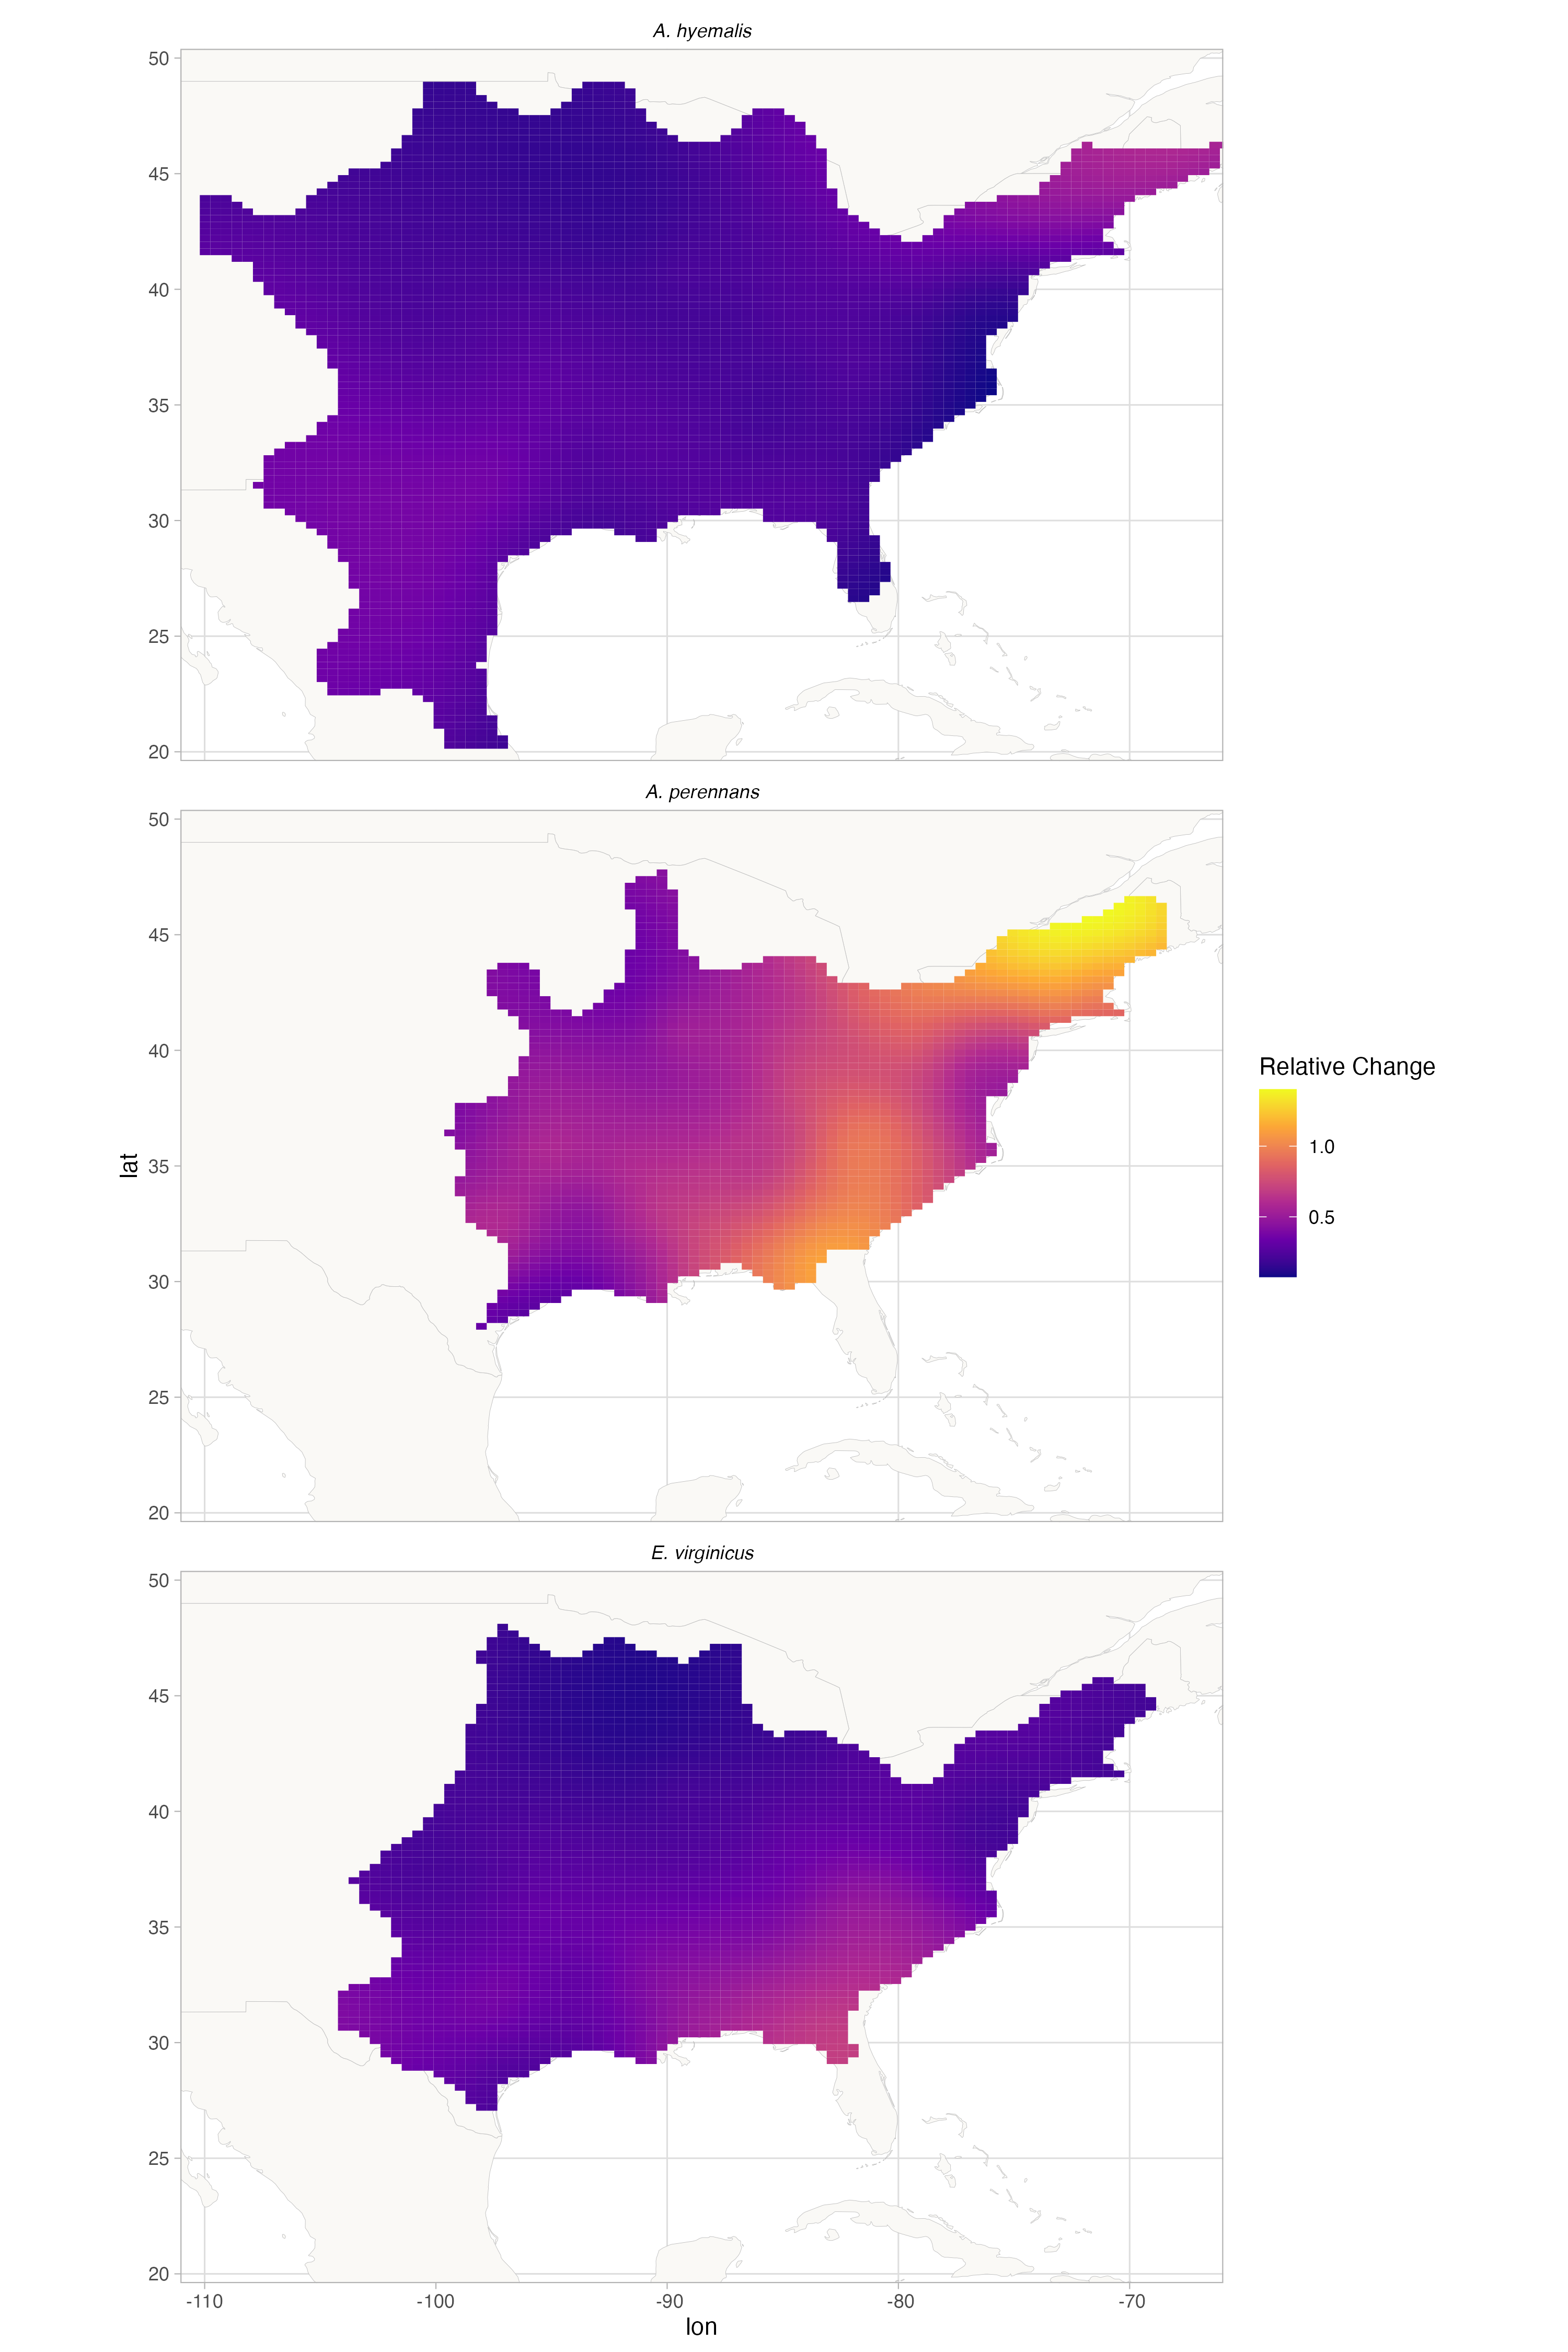
\includegraphics[width = .8\linewidth]{rel_change_plot.png}
	\caption{\textbf{Relative change in predicted prevalence for each host species.} Color indicates the relative change in predicted endophyte prevalence between 1925 and 2020 across the collection range.}
\end{figure}

This revealed locations that were hotspots of change in endophyte prevalence (Fig. 5). 
The overall magnitude of changes were greatest in \emph{A. perennans}, particularly in the northeast and in the south, where endophytes were previously only found at low prevalence (Fig. 3).
\emph{A. hyemalis} and \emph{E. virginicus} experience lower absolute increases in prevalence, yet we can still identify hotspots of change in the northeast for \emph{A. hyemalis} and in the southeast for \emph{E. virginicus}.


\subsubsection*{Performance on test data}
The model adequately predicted mean endophyte prevalence, but underpredicted variance in the contemporary test observations (Fig. 6 A).
The model was able to predict large scale spatial trends in endophyte prevalence, such as declining endophyte prevalence towards western longitudes in \emph{A. hyemalis} (Fig. 6 B-C).
We interpreted this to mean that the model captured regional spatial dynamics, but underpredicts local scale dynamics. We discuss potential model improvements in the Discussion.

\begin{figure}[H]
	\centering
	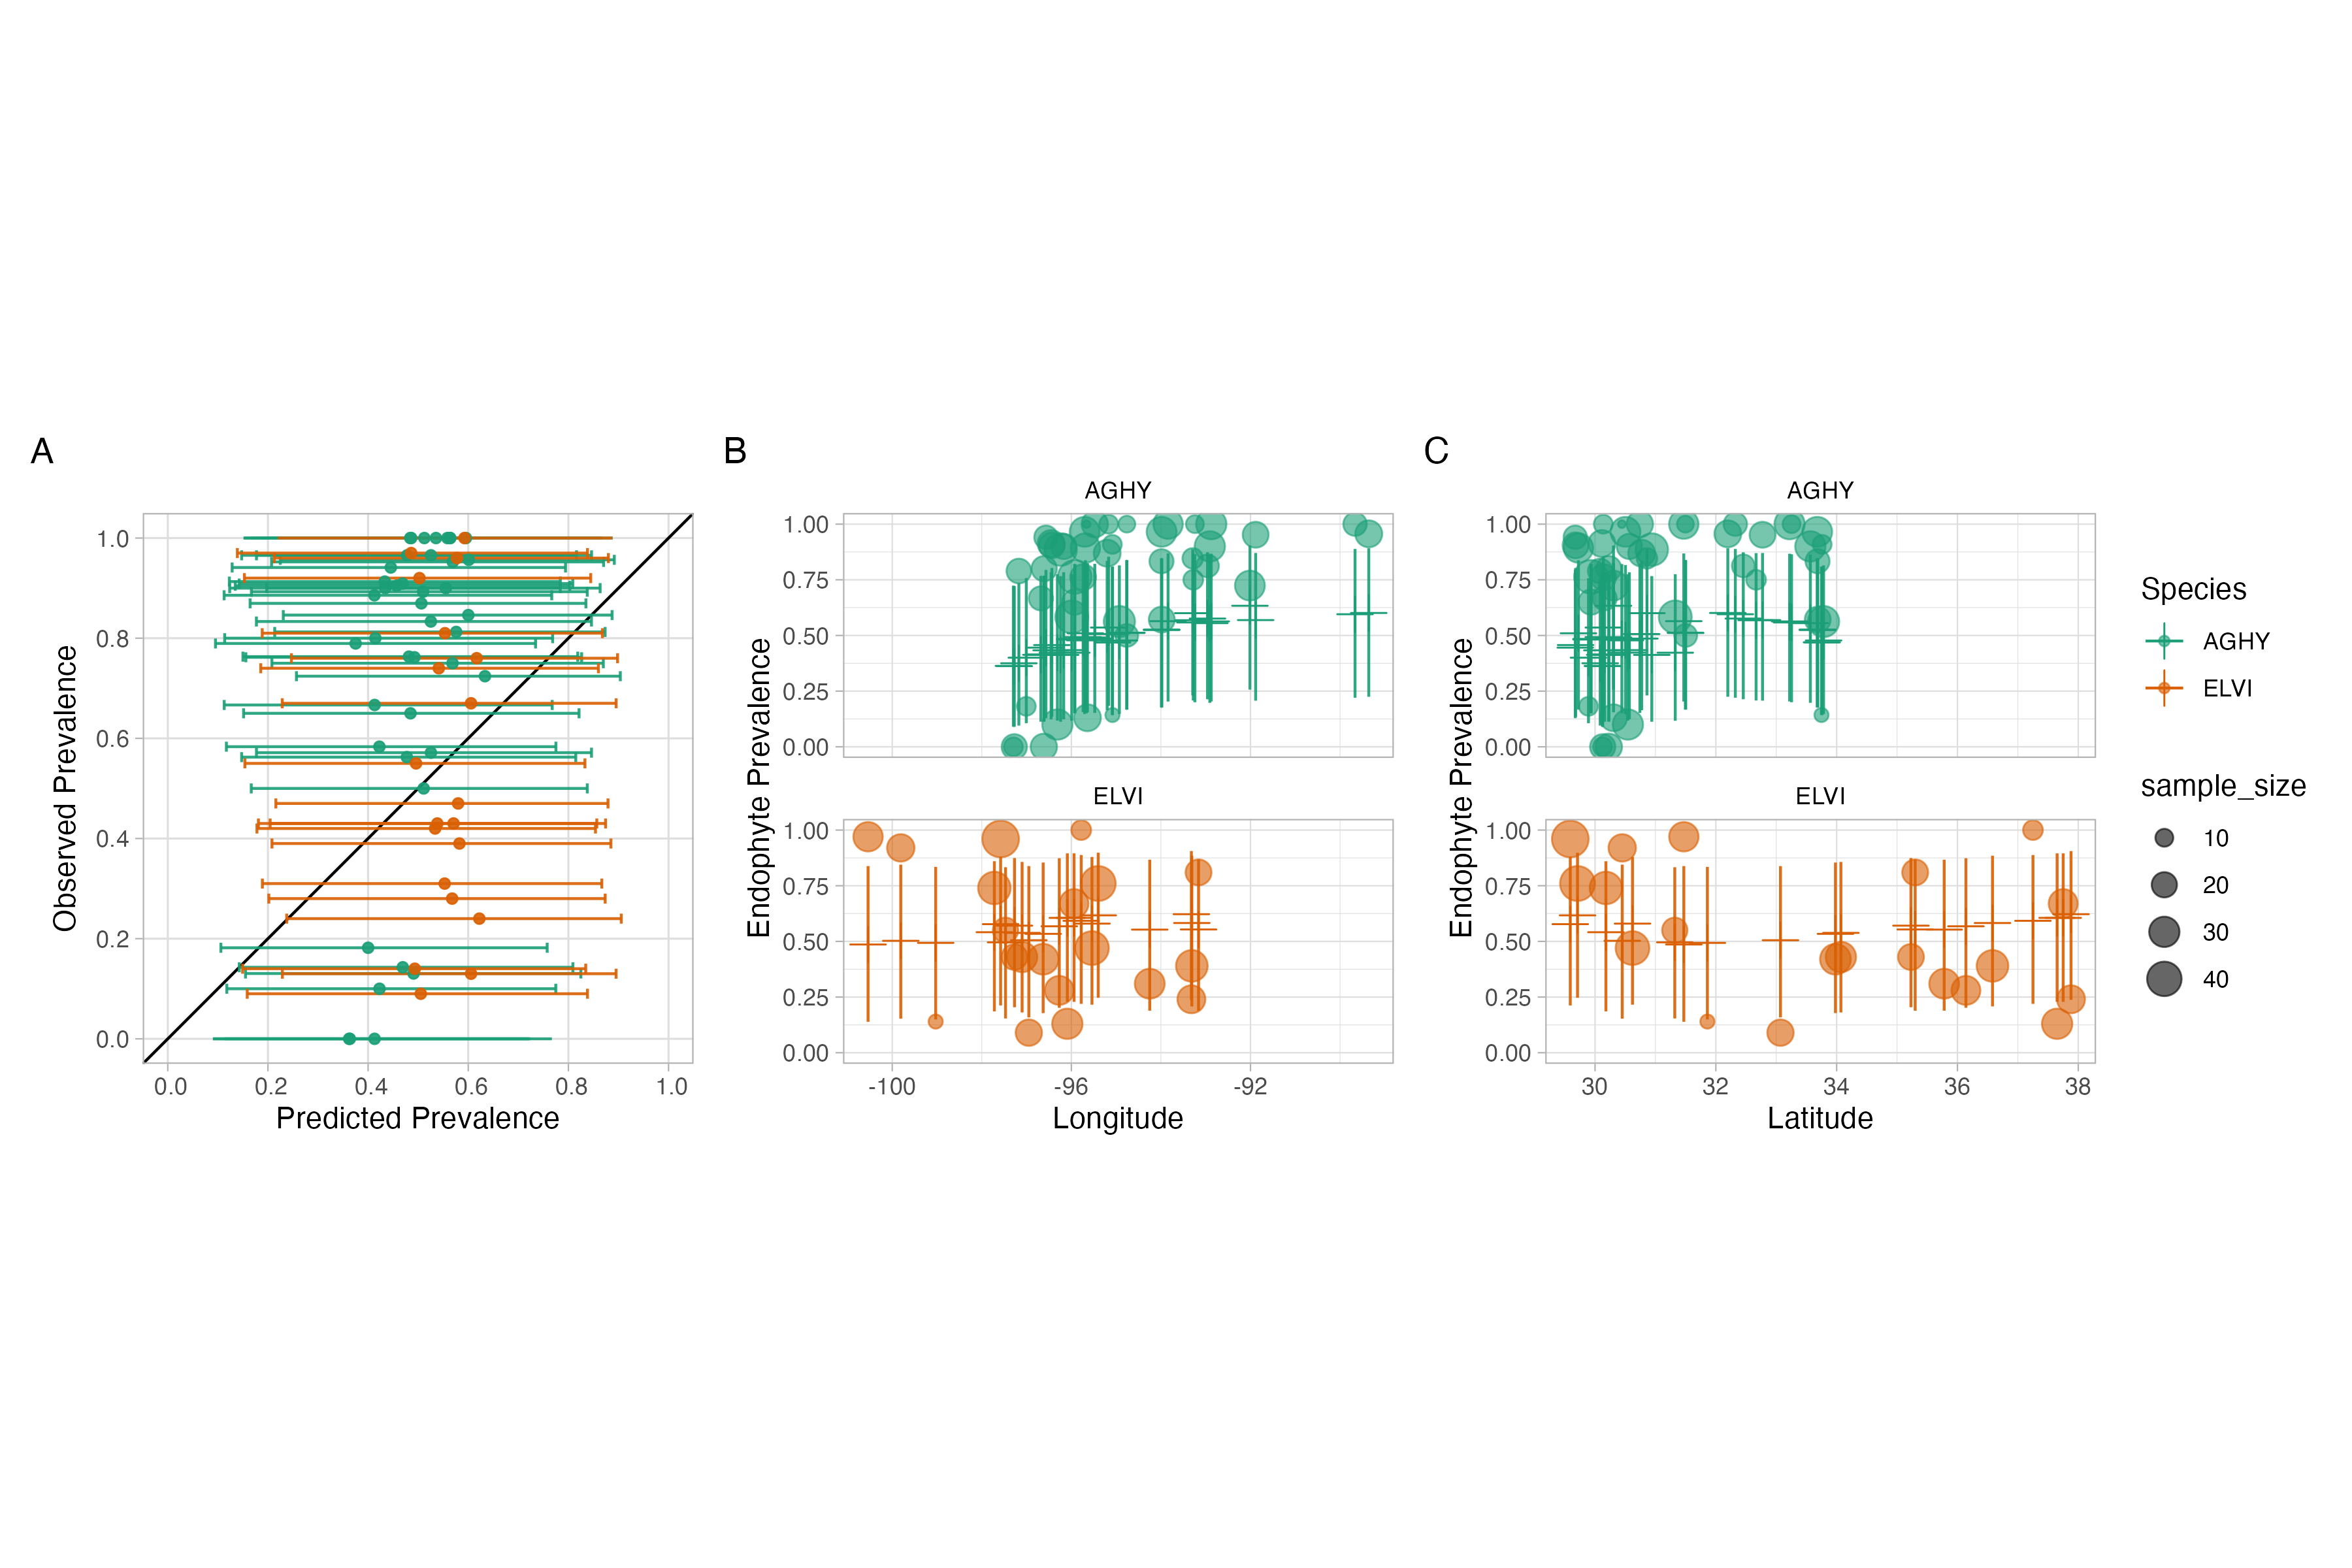
\includegraphics[width = \linewidth]{contemp_test_plot.png}
	\caption{\textbf{Predicted vs observed endophyte prevalence for contemporary test data.} (A) The model, trained on historic herbarium collection data, performed modestly at predicting contemporary endophyte prevalence, as indicated by some overlap of predicted 95\% CI with the 1:1 line, however contemporary test data generally had more variance between populations than model predictions. The model did recapitulate broader regional trends across (B) longitude and (C) latitude. Colors indicate host species, and point size in panels B and C reflect sample sizes of contemporary endophyte population surveys.}
\end{figure}



\subsection*{The role of climate drivers}
\subsubsection*{What is the relationship between variation in temporal trends in endophyte prevalence and changes in climate drivers?}

We found that trends in endophyte prevalence were strongly associated with seasonal climate change drivers (Fig. 6).
For the majority of the study region, the climate has become wetter and cooler over the last century (Fig. A7-A8), a consequence of regional variation in global climate change \cite{ipcc_2021}. 
Within the study region, spatially heterogeneous environmental changes were predictive of changes in endophyte prevalence. 
For example, strong increases in prevalence within \emph{E. virginicus} were most associated with declines in Summer precipitation  (a negative correlation in Fig. 7) as well as with increases in the year-to-year variability of annual temperature (a positive correlation in Fig. 7). 
Changes were also associated with reductions in average annual temperatures, and increases in year-to-year temperature variability.
\emph{A. perennans} endophyte prevalence increased most strongly in regions that experienced reduced spring precipitation and reduced variability in annual temperature.
Although these correlations were weaker, changes in \emph{A. perennans} endophyte prevalence were also associated with increased in increases in annual precipitation and increasing autumn precipitation. 
For \emph{A. hyemalis}, endophyte prevalence increased most strongly in regions that experienced reductions in autumn precipitation variability. 
Correlations using only a subsampling of pixels were qualitatively similar to these results (Fig. A11), suggesting that the patterns we find, particulary the strongest correlations are not spurious associations.

%These associations are in line with expectations that endophyte symbiosis provides drought tolerance to their hosts, particularly during \emph{E. virginicus}'s \tom{summer growing season}{It is a stretch to say that this species has a summer growing season.}. 
%For \emph{A. perennans}, which flowers in the late Summer and Autumn, increases in autumn precipitation along with increases in variability in annual precipitation, were strongly assocated with increasing endophyte prevalence.  
%While this result is contrary to the expectation that endophyte provide drought tolerance, this species typically is associated with wetter microhabitats, and it also \tom{suggests a role for endophytes to play in buffering the negative consequences of demographic variability \citep{lewontin_population_1969}}{I would save for discussion}.  
%For \emph{A. hyemalis}, which flowers in the Spring, changes in endophyte prevalence were more weakly associated with seasonal changes in climate drivers than for the other two species.
%It was, however, the only species' for which greater increases in endophyte prevalence were associated with regions that experienced increases in average annual temperatures.\tom{}{Is this a significant association, however you want to define that? Or could this result have occurred by chance?}

\begin{figure}[H]
	\centering
	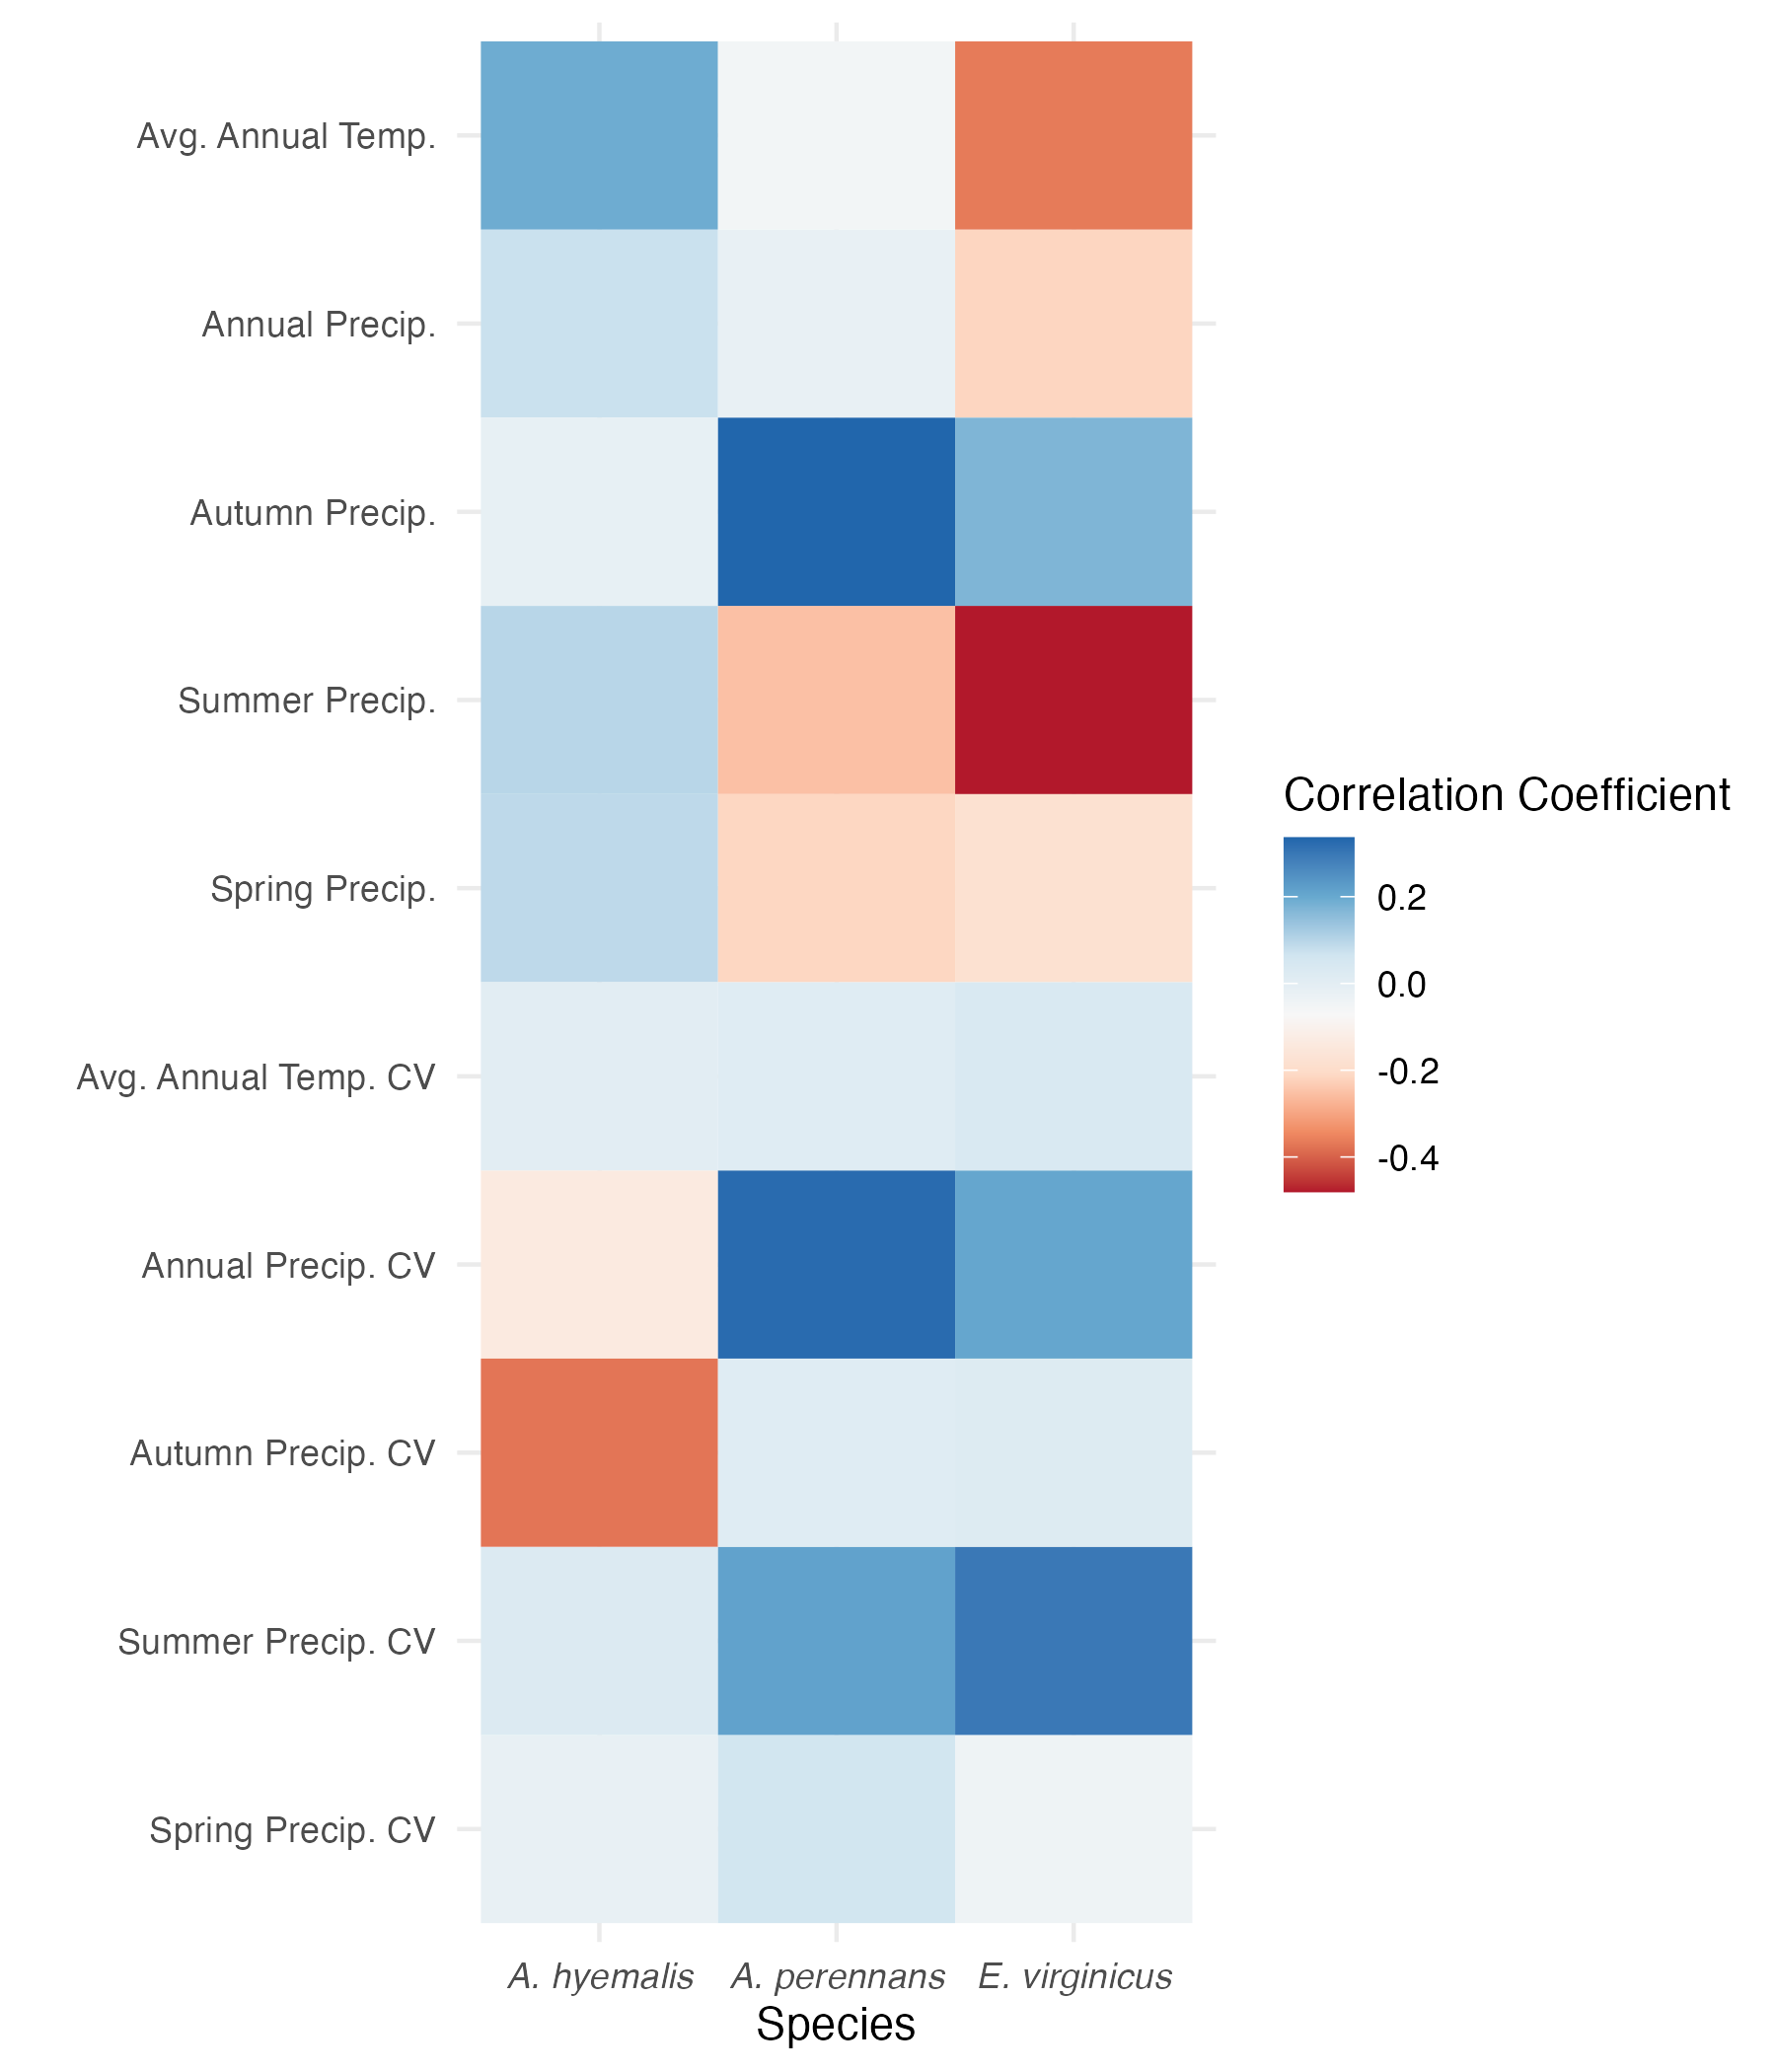
\includegraphics[width = \linewidth]{climate_corr_heatmap.png}
	\caption{\textbf{Correlations between changes in climate drivers and changes in endophyte prevalence.} Color denotes the Spearman correlation coefficient between the relative rate of change in endophyte prevalence and the change in annual mean temperature ($^oC$) and total annual and seasonal precipitation (mm), as well as the change in the coefficient of variation of each climate driver. Positive correlation coefficients indicate that greater increases in a climate driver were associated with larger increases in endophyte prevalence, while negative values indicate that . Asteriks denote correlation coefficients $> .3$ or $< -.3$.}
\end{figure}

\section*{Discussion}
Our examination of historic plant specimens revealed a cryptic biotic reponse to climate change. 
For the three host species we examined, there have been clear increases in fungal endophyte prevalence over the last two centuries.
Increases in prevalence of \emph{Epichloë}, which are vertically transmitted, can potentially be interpreted as adaptive changes that improve the fitness of their hosts under stressful conditions.
This interpretation is in line with theory predicting that the positive fitness feedback caused by vertical transmission leads beneficial symbionts to rise in prevalence within a population \cite{fine1975vectors}.
We found that trends in endophyte prevalence varied across the collection range of each species in assocation with observed changes in climate drivers, suggesting that the endophytes have contributed to host resilience under environmental change.
Taken together, this suggests a strengthening of the mutualism over the last two centuries.


Differences between the responses of each host species underscore that while all of these $C_3$ grasses share similar broad-scale distributions, each engages in unique biotic interactions and has unique niche requirements.
We identified hotspots of change in the northeast and south for \emph{A. perennans}, which experienced the strongest absolute changes in endophyte prevalence (Fig. 5). 
Based on previous work demonstrating that endophytes can shield their hosts from drought stress \cite{decunta2021systematic}, we generally predicted that drought conditions could be a driver of increasing endophyte prevalence. 
In line with this expectation, increasing prevalence for this species was associated with decreasing precipitation, most strongly with spring-season declines (Fig. 7). 
\emph{A. perennans} typically blooms in the autumn.
Endophytes could be playing a role helping hosts weather spring-season droughts while the species is dormant. 
It may be useful to investigate whether lagged climate effects are important predictors of host fitness in this system \cite{evers2021lagged}. 
To our knowledge, the response of the symbiosis in \emph{A. perennans} to drought has not been examined experimentally, but in a greenhouse experiment, endophytes had a positive effect on host reproduction under shaded, low-light conditions \citep{davitt2010costs}. 
\emph{Epichloë} endophytes have been connected to a suite of non-drought related fitness benefits including herbivore protection \citep{brem2001epichloe}, salinity resistence \citep{wang2020effects}, and mediation of the soil microbiome \citep{roberts2015rhizosphere} 
These effects are potentially mediated by the diverse bioactive alkaloids and other signaling compounds they produce \citep{saikkonen2013chemical}.
The strong increase in symbiotic \emph{A. perennans} could be explained, at least in part, by these diverse benefits. 
\emph{A. hyemalis} experienced smaller overall changes in endophyte prevalence, and these changes were only weakly related to changes in climate drivers. 
This result was surprising given previous work demonstrating drought benefits in a greenhouse manipulation with this species \citep{davitt2011understanding} that led us to expect  that endophyte prevalence should similarly increase at a greater rate in regions that have experienced increasing drought.
It is possible that the study region has not experienced a magnitude of climate change great enough to cause larger changes in endophyte prevalence for this species. 
Weak associations with drought could also be explained by climate-driven changes in the rate of imperfect transmission (the generation of non-symbiotic offspring from symbiotic hosts), which could counterbalance endophyte-mediated fitness benefits \citep{donald2021context}. 
For \emph{E. virginicus}, which also experienced more modest changes in endophte prevalence overall, we found a strong relationship between temporal trends and  changes in the mean and variability of temperature, as well as with decreases in summer precipitation.
Surveys by \citet{sneck2017variation}, used as part of the test data in this study, identified a drought index (SPEI) that integegrates precipitation with estimated evapotranspiration as an important predictor of endophyte prevalence.
While we show consistent increasing trends in prevalence between the three species, the mechanisms that explain these changes may be diverse and idiosyncratic. 

Our spatially-explicit model predicted regions of both high and low endophyte prevalence, suggesting that symbiotic and non-symbiotic host plants have overlapping, but non-identical niche requirements.
Endophytes fitness benefits potentially explain the spatial distribution of prevalence by allowing their hosts to persist in environments where they otherwise could not \citep{afkhami2014mutualist, kazenel2015mutualistic}.
For example, fitness benefits of the symbiosis could explain high predicted prevalence in \emph{E. virginicus} towards the north or in \emph{A. hyemalis} towards its range center coinciding with strong environmental gradients.
Previous population surveys for endophytes, which were used as test data for our model, found similar latitudinal trends in prevalence in these species \citep{sneck2017variation,rudgers2009benefits}, but at smaller scales. 
While the model recreated these large-scale spatial trends, test data was more variable. 
Using test data to validate our model predictions allows us to evaluate places to improve the model's ability to perform well at out-of-sample prediction, which will be particularly important for predicting host and symbiont niche-shifts under future climate change.
Lack of information on local variability may simply be a feature of data derived from herbarium specimens. 
Even though they are samples from local populations, that are single specimens that are aggregated over in broad-scale model estimates.
Poor predictive ability at local scales in this grass-endophyte system is not surprising, as previous studies have found that local variation, even to the scale of hundreds of meters can structure endophyte-host niches \cite{kazenel2015mutualistic}. 
\citet{sneck2017variation} also identified host genotype as an important predictor of endophyte prevalence in \emph{E. virginicus}.
Other studies have found factors including land-use history \cite{vikuk2019infection} and the biotic environment, including herbivory \cite{rudgers2016long}, to be important predictors of endophyte ecology.
Incorporating available climatic and soil layers as covariates is an obvious first step that could improve predictions.
Towards the goal of predicting the microbial symbioses dynamics under climate change, models that integrate data from local and regional scales would be an important step to bridge the gap that often exists between large but broad bioclimatic and biodiversity data and small but local data on biotic interactions.  \cite{miller2019recent, isaac2020data}


Our analysis advances the use of herbarium specimens in global change biology in two ways. 
First and foremost, this is the first study to link long-term changes in microbial symbioses to changes in climate using specimens from natural history collections.
The responses of microbial symbioses are a rich target for future studies within museum specimens, particularly those that take advantage of advances in sequencing technology.
While we used relatively coarse presence/absence data based on fungal morphology, other studies have examined historic plant microbiomes using molecular sequencing and sophisticated bioinformatics techniques, but these studies have so far been limited to relatively few specimens at limited spatial extents \cite{yoshida2015computational, heberling2019utilizing, bieker2020metagenomic, gross2021hidden, bradshaw2021global}. 
Continued advances in capturing historic DNA and in filtering out potential contamination during specimen storage \citep{daru2019novel, bakker2020herbarium, raxworthy2021mining} will be imperative in the effort to scale up these efforts. 
This scaling up will be essential to be able to quantify changes not just in the prevalence of symbionts, but also in symbionts' intraspecific variation and evolutionary responses to climate change, as well as  in changes in the wider microbial community. 
Answering these questions as well as the unknown questions that future researchers may ask also reiterates the value in capturing meta-information during ongoing digitization efforts at herbaria around the world and during the accession of newly collected specimens \citep{lendemer2020extended}.
Second, we accounted for several potential biases in the data observation process that may be common to many collections-based research questions by using a spatially-explicit random effects model. 
Spatial autocorrelation \cite{willems2022forest}, potential biases introduced by the sampling habits of collectors \citep{daru2018widespread}, and variation between contemporary researchers during the collection of trait data, if not corrected for could lead to biased inference about the strength and direction of historic change.
Previous studies that have quantified the effects of collector biases typically find them to be small  \cite{davis2015herbarium,meineke2019herbarium}, and we similarly did not find that collector has a strong effect on the results of our analysis.
Fitting this model in a Bayesian framework allows for full propagation of uncertainty.

Ultimately, a central goal of global change biology is to generate predictive insights into the future of natural systems. 
While this survey of historic endophyte prevalence is necessarily correlative, it serves as a foundation to develop better predictive models of the response of microbial symbioses to climate change. 
Combining the insights from this type of regional-scale survey with field experiments and physiological data could be invaluable. 
While we found that climate is strongly correlated with endophytes' temporal responses, we do not know why trends in prevalence were weak in some areas or how endophytes would respond to more extreme changes in climate.
For example, transplanting symbiotic and non-symbiotic plants beyond the range edge of \emph{A. hyemalis} could tell us whether persistent low endophyte prevalence in that area is a result of environmental conditions that lead the symbiosis to negative fitness consequences, or is a result of some historical contingency or dispersal limitation that has thus far limited the presence of symbiotic hosts from a region where they would otherwise flourish and provide resilience.
While we observed evidence of mutualism resilience, more extreme environmental changes than those observed in our study could potentially push one or both partners beyond their physiological limit, leading to the collapse of the mutualism. 
Our analysis thus far is agnostic to changes in the distributions of hosts. 
Mechanistic models could connect the responses of both host and symbionts to abiotic climate drivers integrating dispersal processes. 
Beyond host-microbe symbioses, building these types of models would work towards quantitatively attributing biotic responses to anthropogenically driven climate change, similar to methods in climate science and economics \citep{stott2010detection, carleton2016social}.
%Elymus genotype
%Agrostis weedy



	%%%%%%%%%%%%%%%%%%%%%
	% Acknowledgments
	%%%%%%%%%%%%%%%%%%%%%
	% You may wish to remove the Acknowledgments section while your paper 
	% is under review (unless you wish to waive your anonymity under
	% double-blind review) if the Acknowledgments reveal your identity.
	% If you remove this section, you will need to add it back in to your
	% final files after acceptance.
	
	\section*{Acknowledgments}
	We thank Jessica Budke for help in drafting our initial destructive sampling plan, and to the many members of herbarium staff who facilitated our research visits, as well as to the hundreds of collectors who contributed to the natural history collections. 
	Several high schooler and undergraduate researchers contributed to data collection, including A. Appio-Riley, P. Bilderback, E. Chong, K. Dickens, L. Dufresne, B. Gutierrez, A. Johnson, S. Linder, E. Scales, B. Scherick, K. Schrader, E. Segal , G. Singla, and M. Tucker.
	This research was supported by funding from National Science Foundation (grants 1754468 and 2208857) and by funding from the Texas Ecolab Program.


	%%%%%%%%%%%%%%%%%%%%%
	% Statement of Authorship
	%%%%%%%%%%%%%%%%%%%%%
	% This section should also be commented out while your MS is undergoing
	% double-blind review. The specifics should of course be adapted to
	% your paper, but the paragraph below gives some hints of possible
	% contributions.
	
	\section*{Statement of Authorship}
	

	
	\section*{Data and Code Availability}
	
	On initial submission, you may use this section to provide a URL for editors and reviewers that is `private for peer review'. After acceptance, this section must be updated with correct, working DOIs for data deposits (typically on the Dryad Digital Repository, ) and code deposits (such as in Zenodo). 
	
	\section*{Appendix A}
	\renewcommand{\thefigure}{A\arabic{figure}}
	\setcounter{figure}{0}
	
		\renewcommand{\thetable}{A\arabic{table}}
	\setcounter{equation}{0}  % reset counter 
	\setcounter{figure}{0}
	\setcounter{table}{0}
	
	\begin{figure}[H]
		\centering
		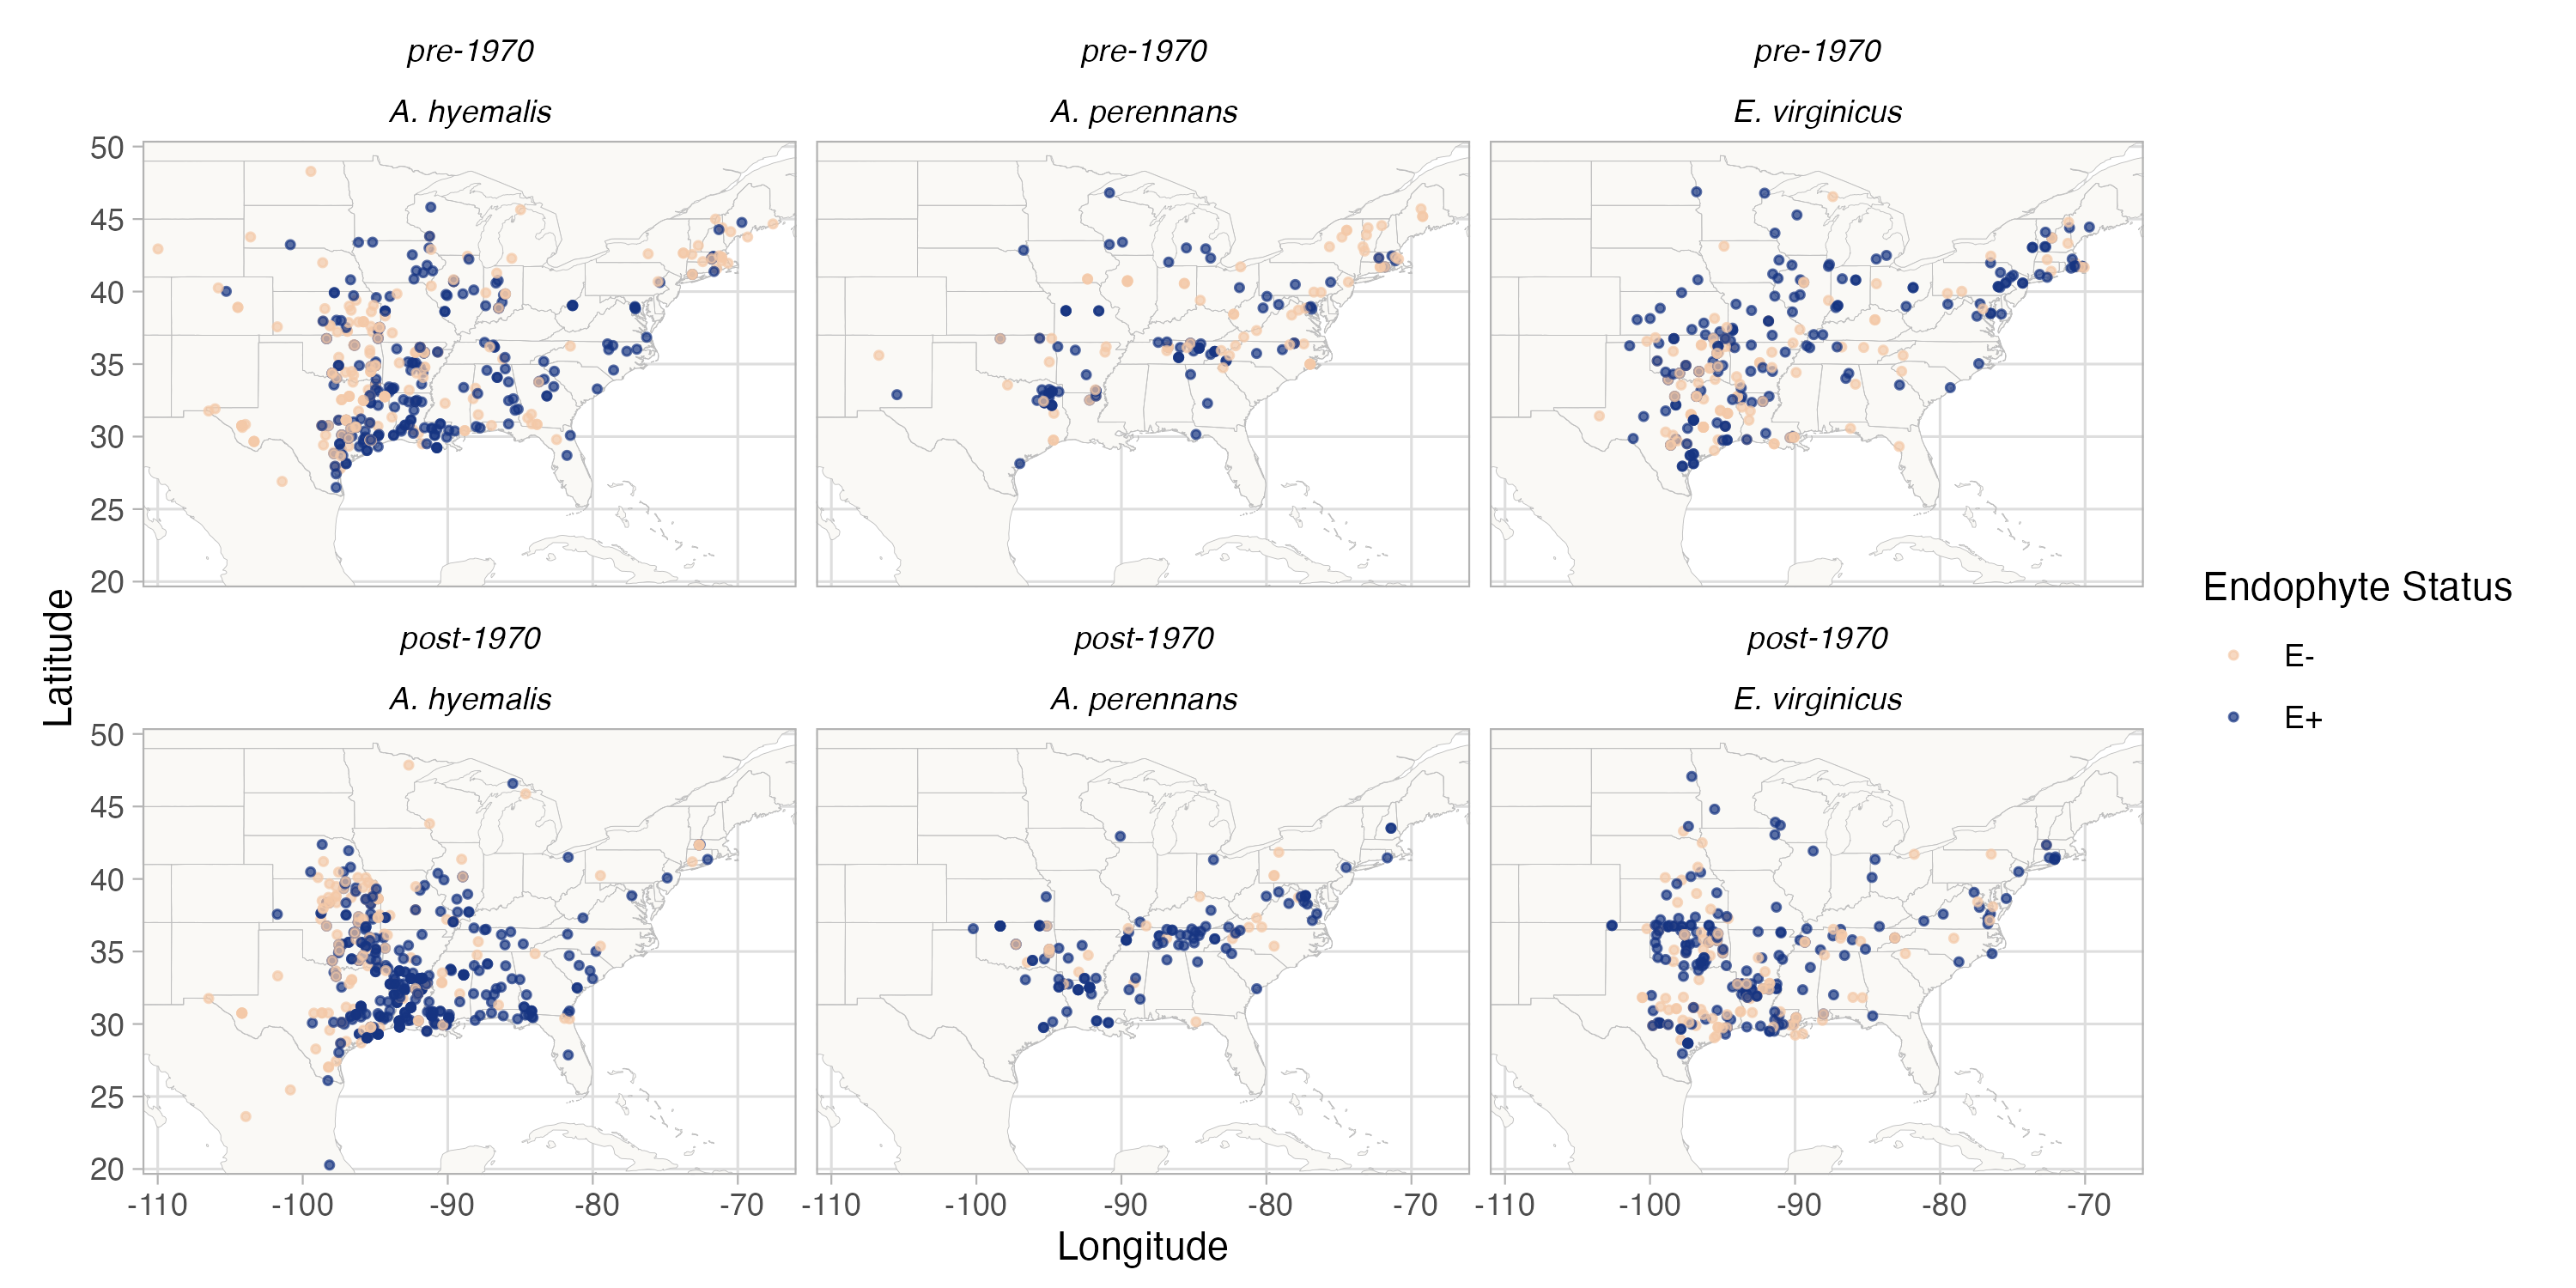
\includegraphics[width = \linewidth]{endo_status_map.png}
		\caption{\textbf{Endophyte presence/absence in specimens of each host species.} Points show collection locations colored according to whether the specimen contained endophytes ( E+; blue points) or did not contain endophytes (E-, tan points) and are faceted based on collection period.}
	\end{figure}
	
	\begin{figure}[H]
		\centering
		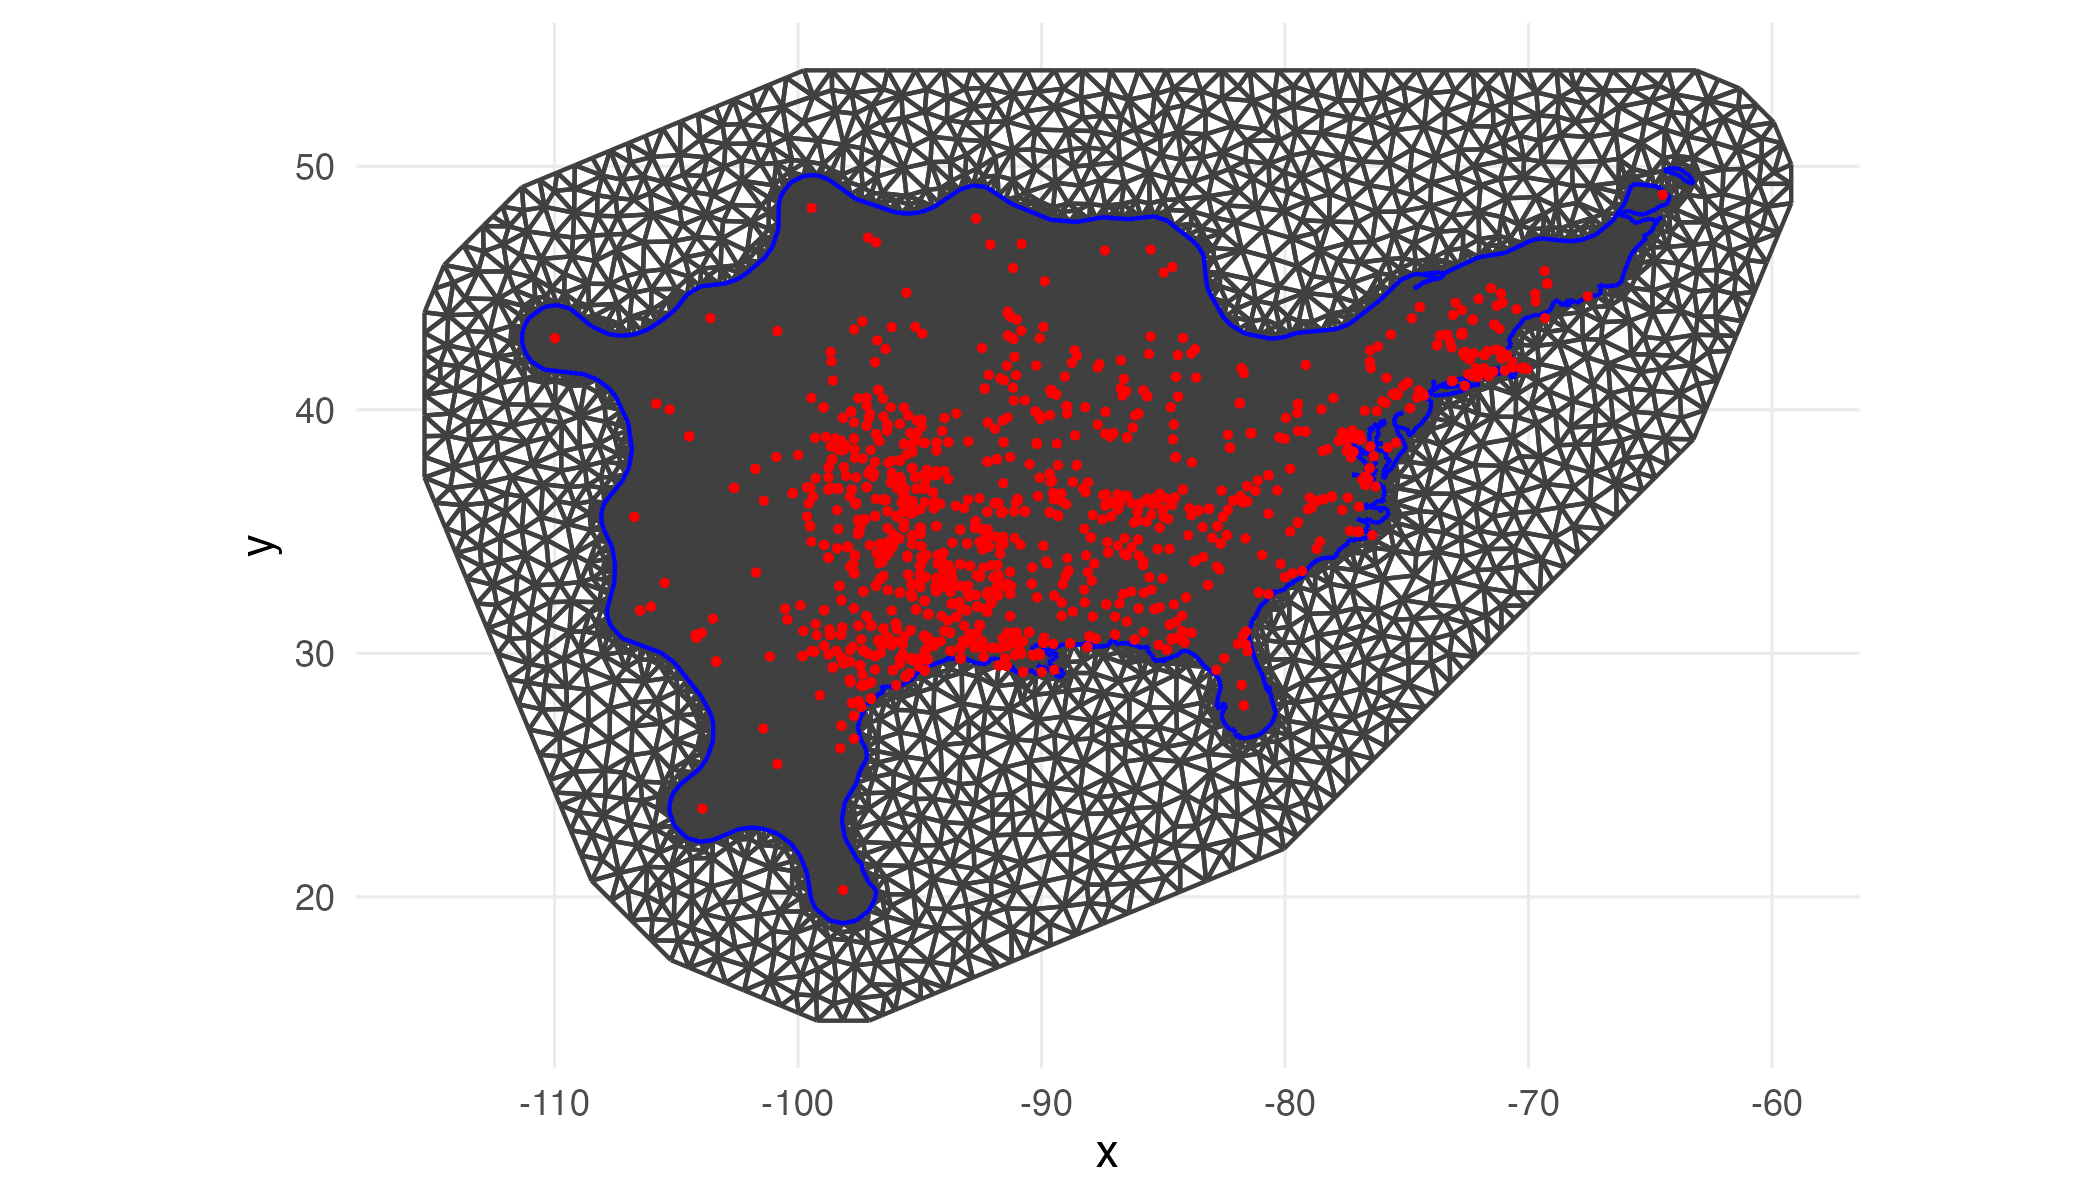
\includegraphics[width = \linewidth]{mesh_plot.png}
		\caption{\textbf{Delauney triangulation mesh used to estimate spatial dependence between data points}. Grey lines indicate edges of triangles used to define distances between observations. Red points indicate locations of sampled herbarium specimens, and the blue outlines show the international borders used to define the edge of the mesh along coastlines.}
	\end{figure}

\begin{figure}[H]
	\centering
	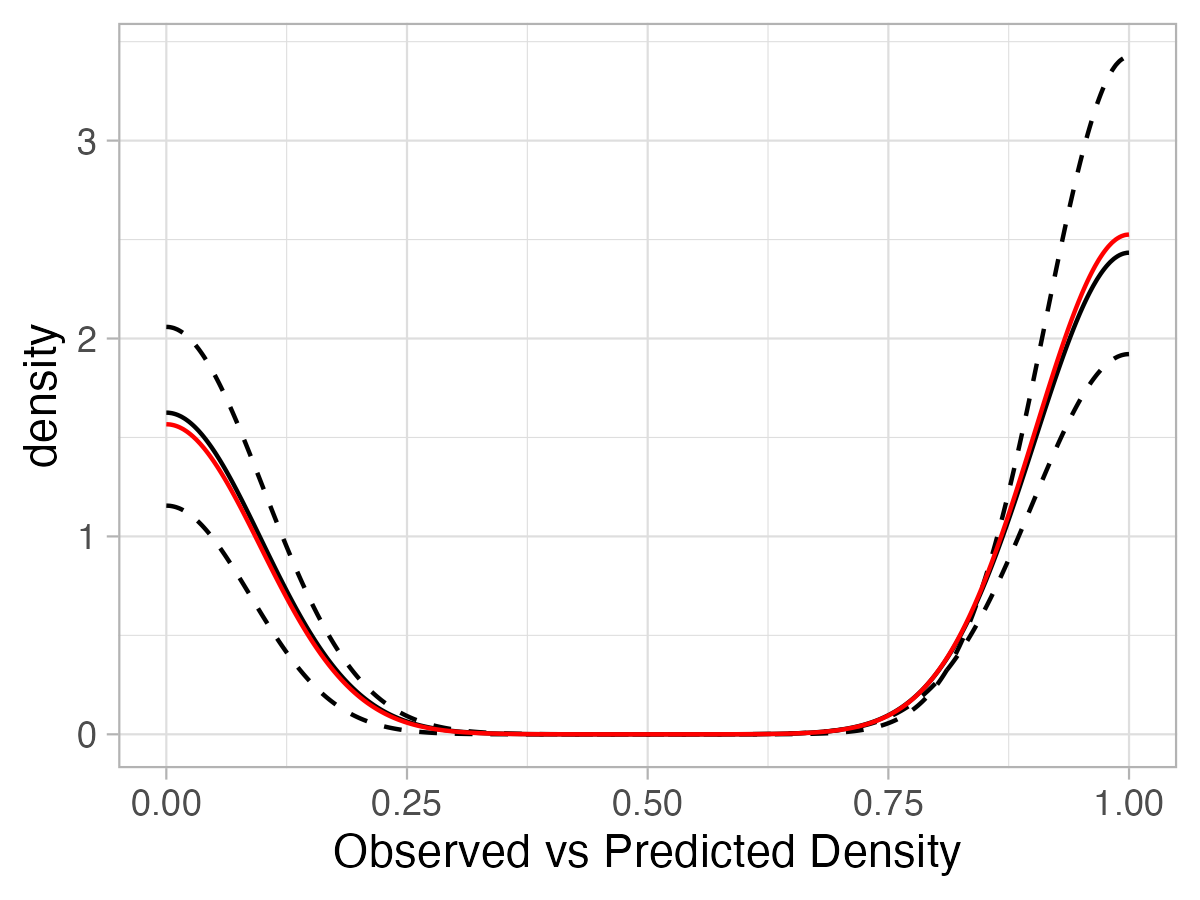
\includegraphics[width = .8\linewidth]{density_plot.png}
	\caption{\textbf{Consistency between real data and simulated values indicate that the fitted model accurately describes the data}. Graph shows density curves for the observed data (red) along with the mean(solid) and 95\% CI (dashed) of simulated values (black).}
\end{figure}

	
	\begin{figure}[H]
		\centering
		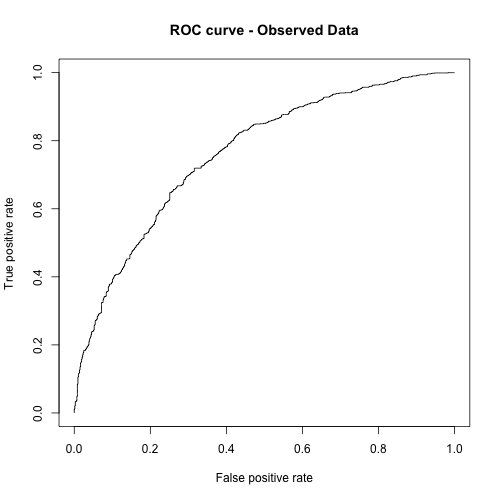
\includegraphics[width = .5\linewidth]{ROC_plot.png}
		\caption{\textbf{ROC plot showing model performance classifying observations according to endophyte status.} The curves show adequate model performance for observed (top) and test (bottom) data. The AUC for each is 0.77.}
	\end{figure}

\begin{figure}[H]
	\centering
	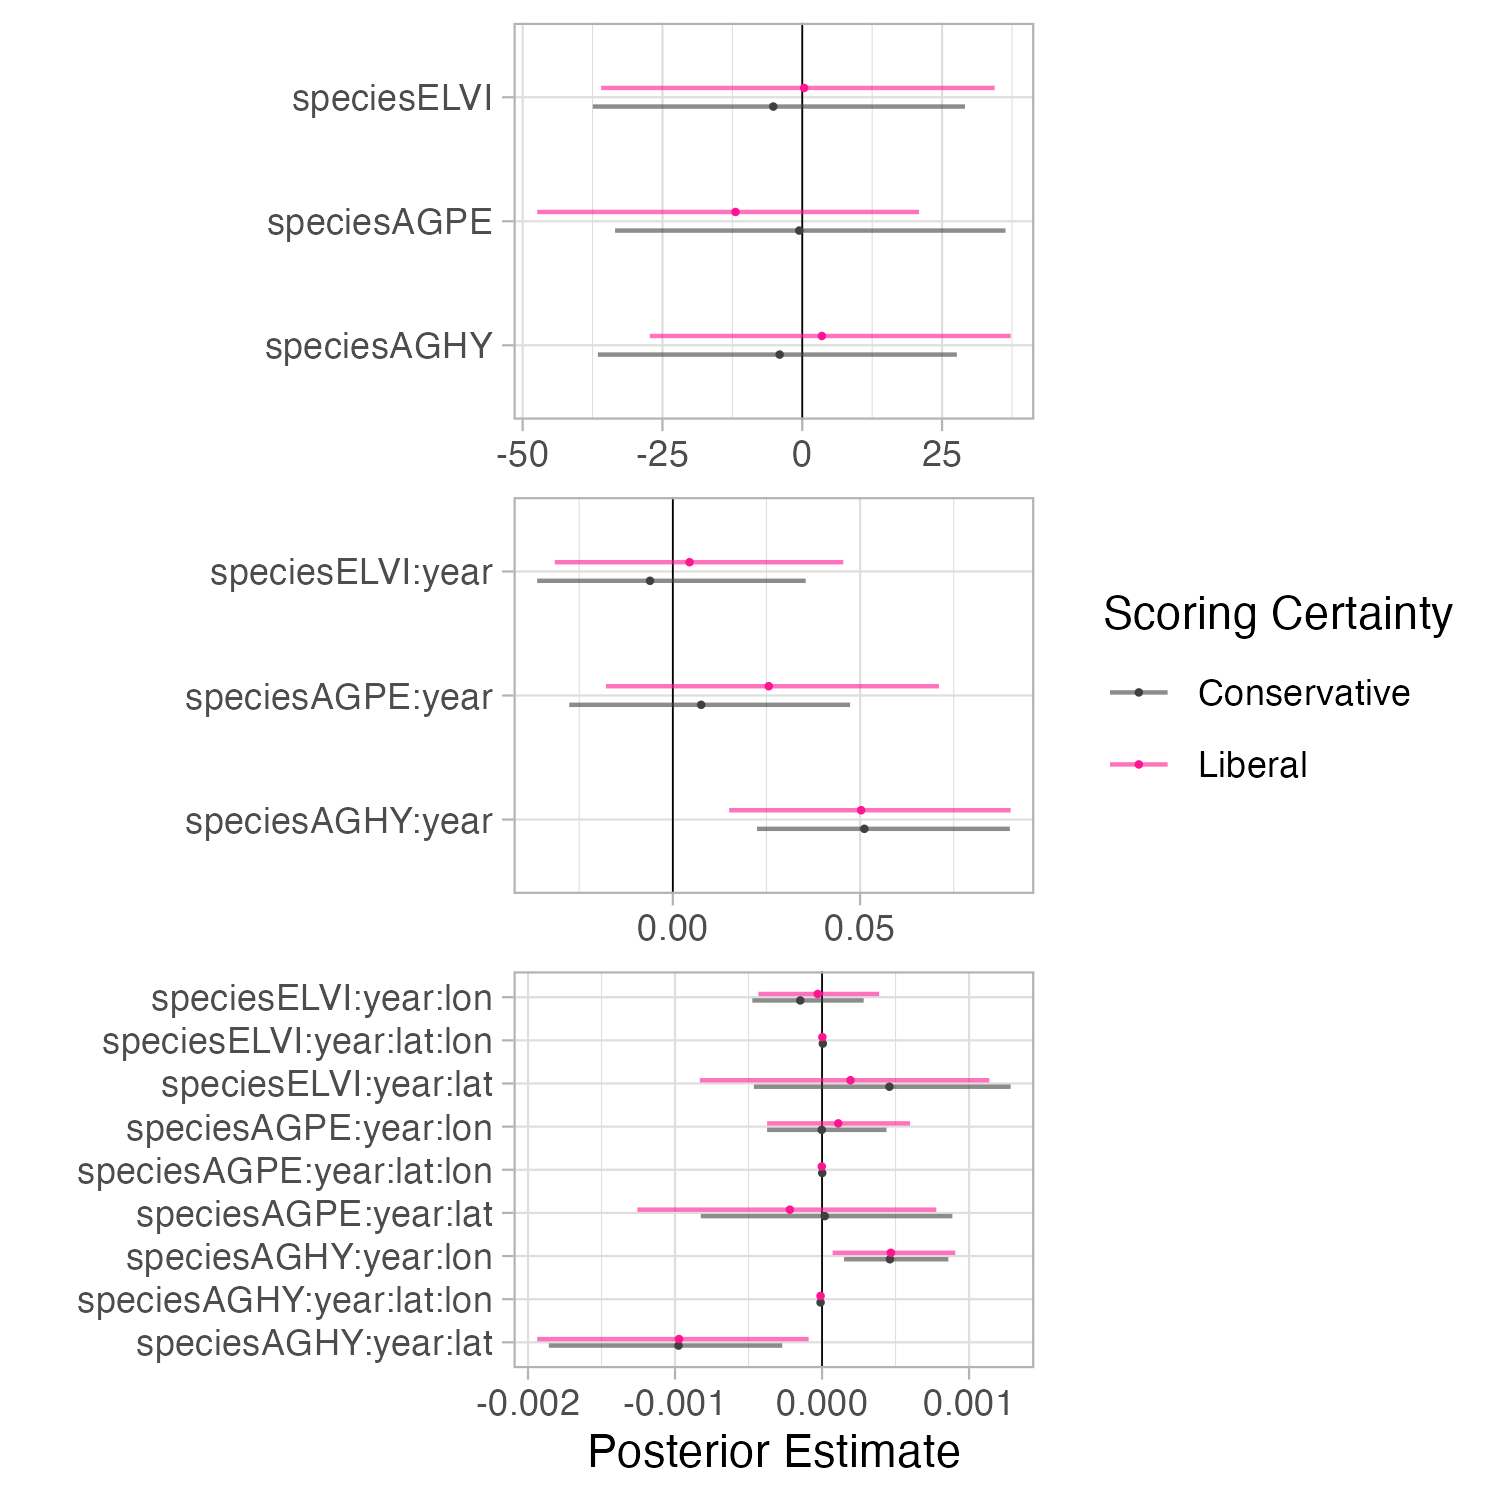
\includegraphics[width = \linewidth]{fixed_plot.png}
	\caption{\textbf{Comparison of posterior estimates of fixed effects when using Liberal or Conservative endophyte scores.}}
\end{figure}

\begin{figure}[H]
	\centering
	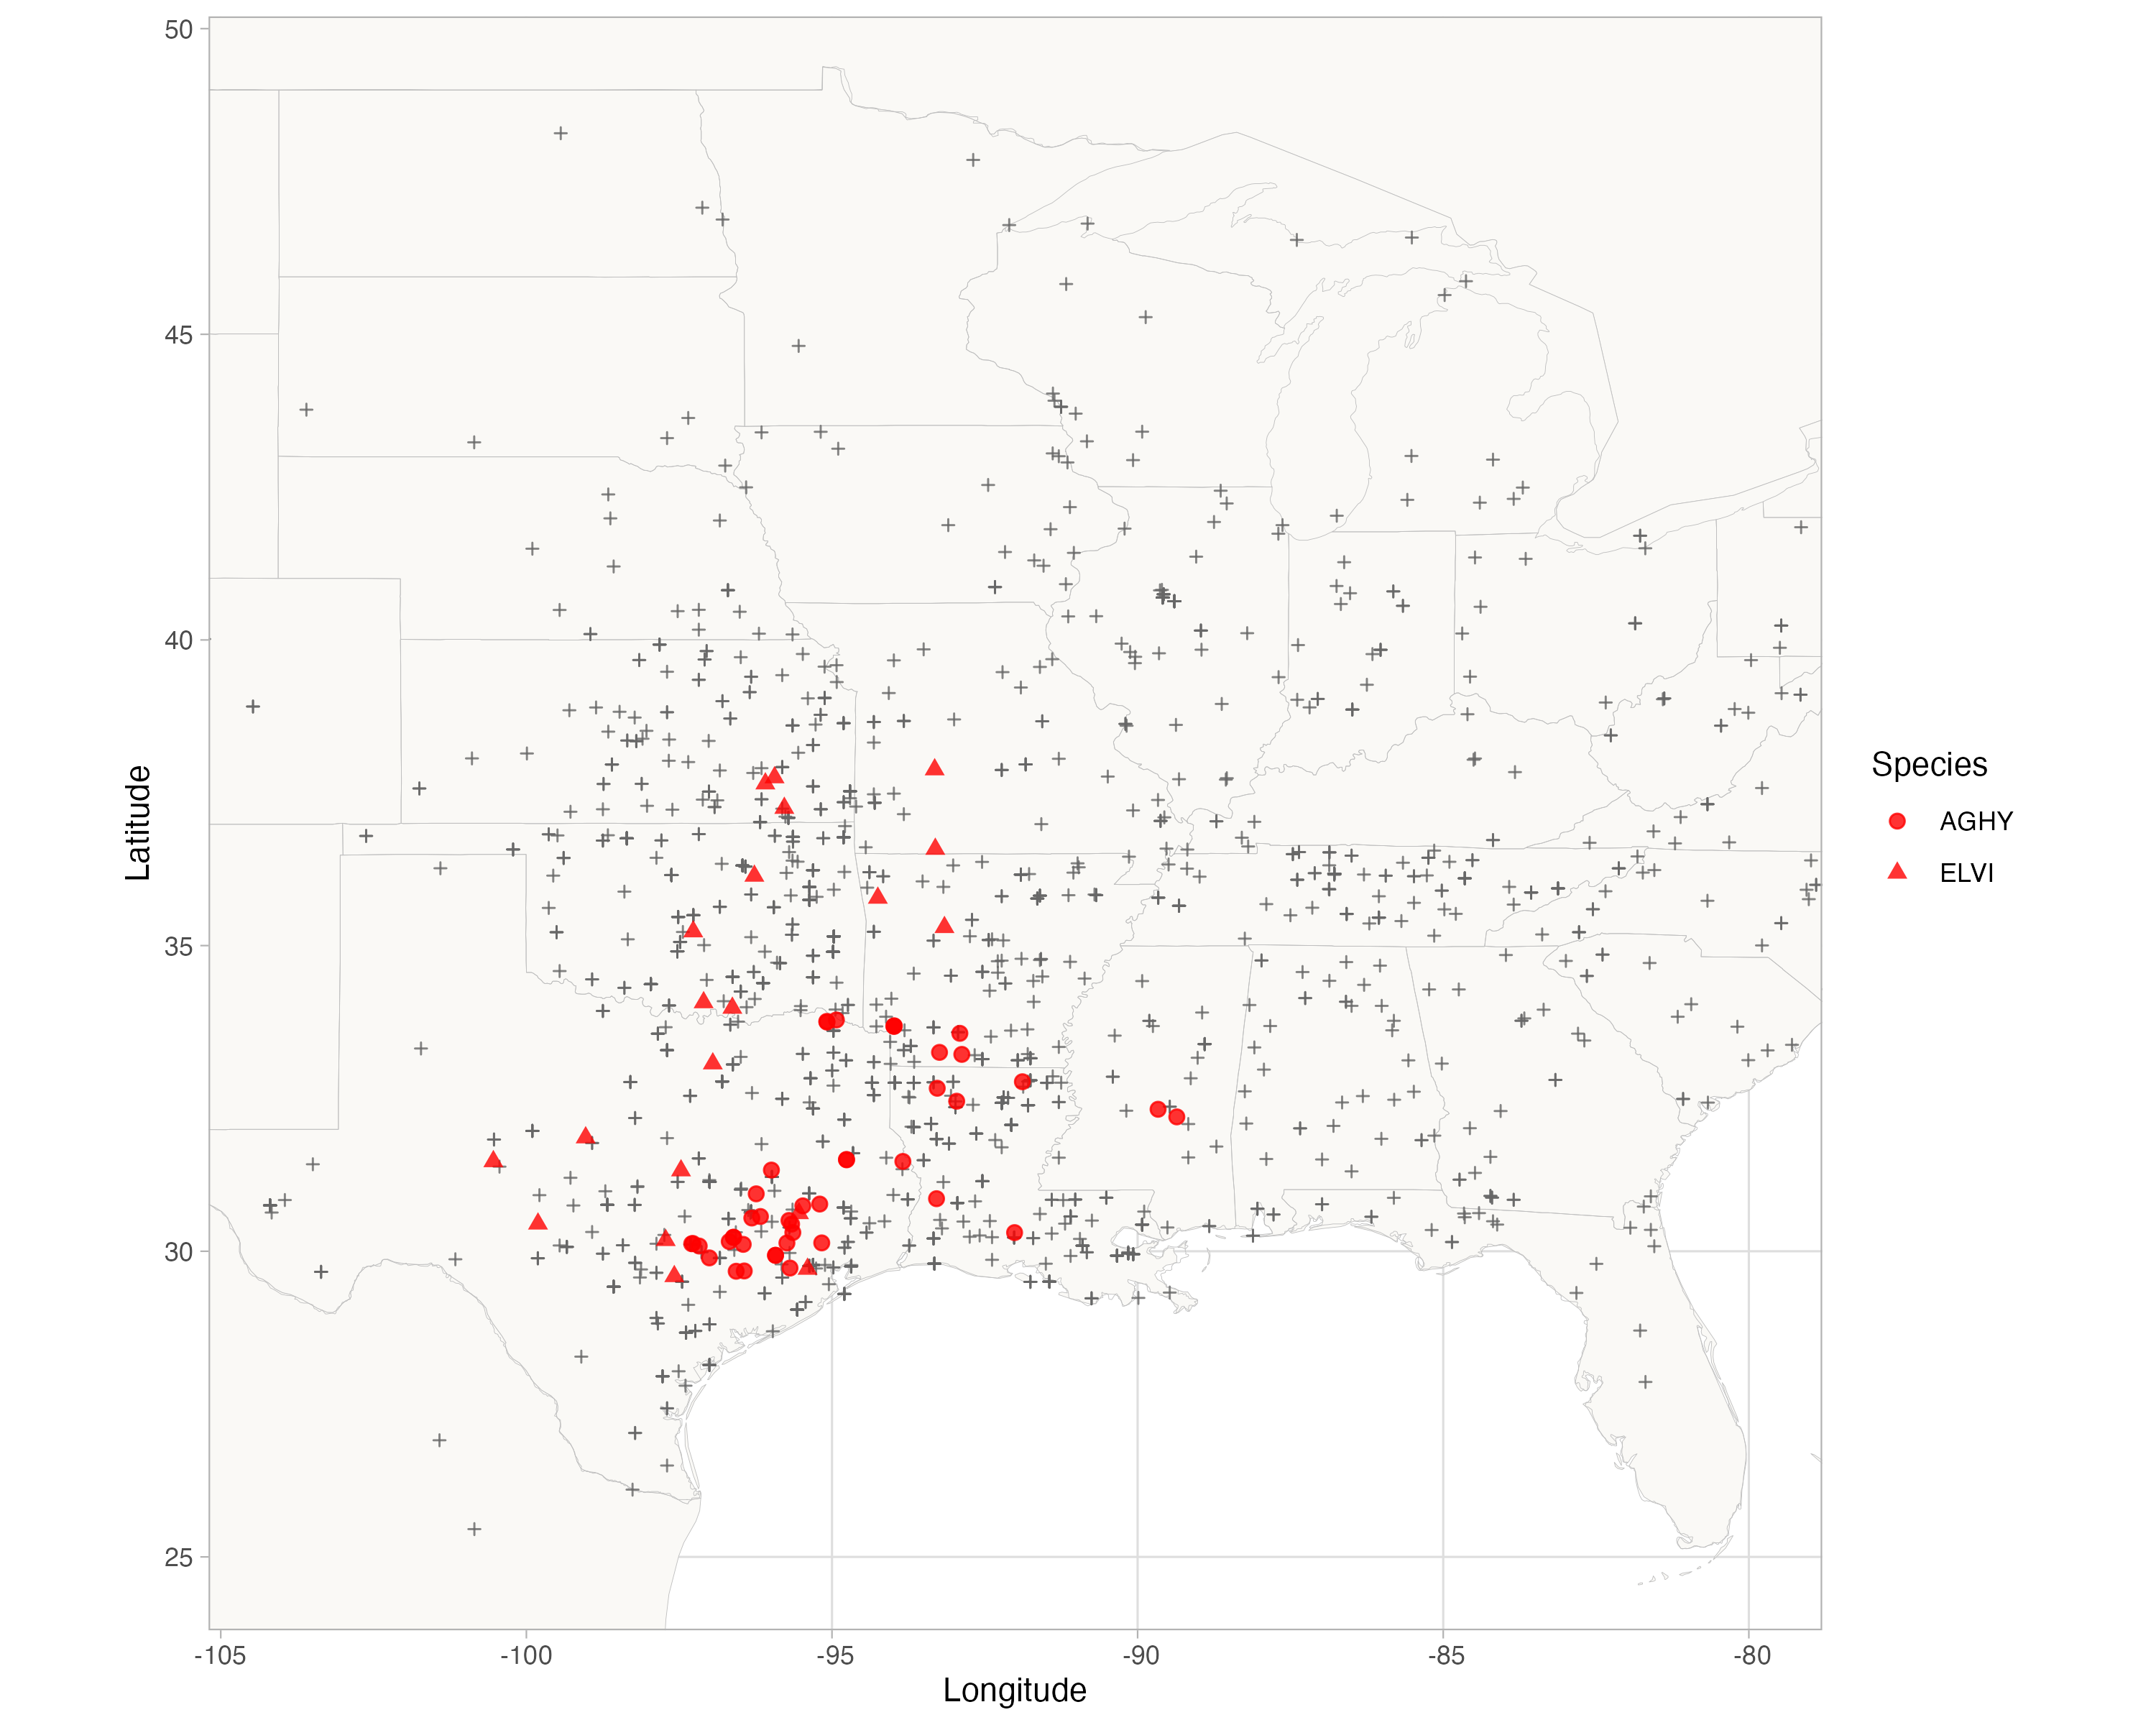
\includegraphics[width = \linewidth]{test_data_map.png}
	\caption{\textbf{Locations of contemporary surveys of endophytes in \emph{A. hyemalis} used as "test" data (red points), relative to the historical collection data (black crosses).}}
\end{figure}

	\begin{figure}[H]
	\centering
	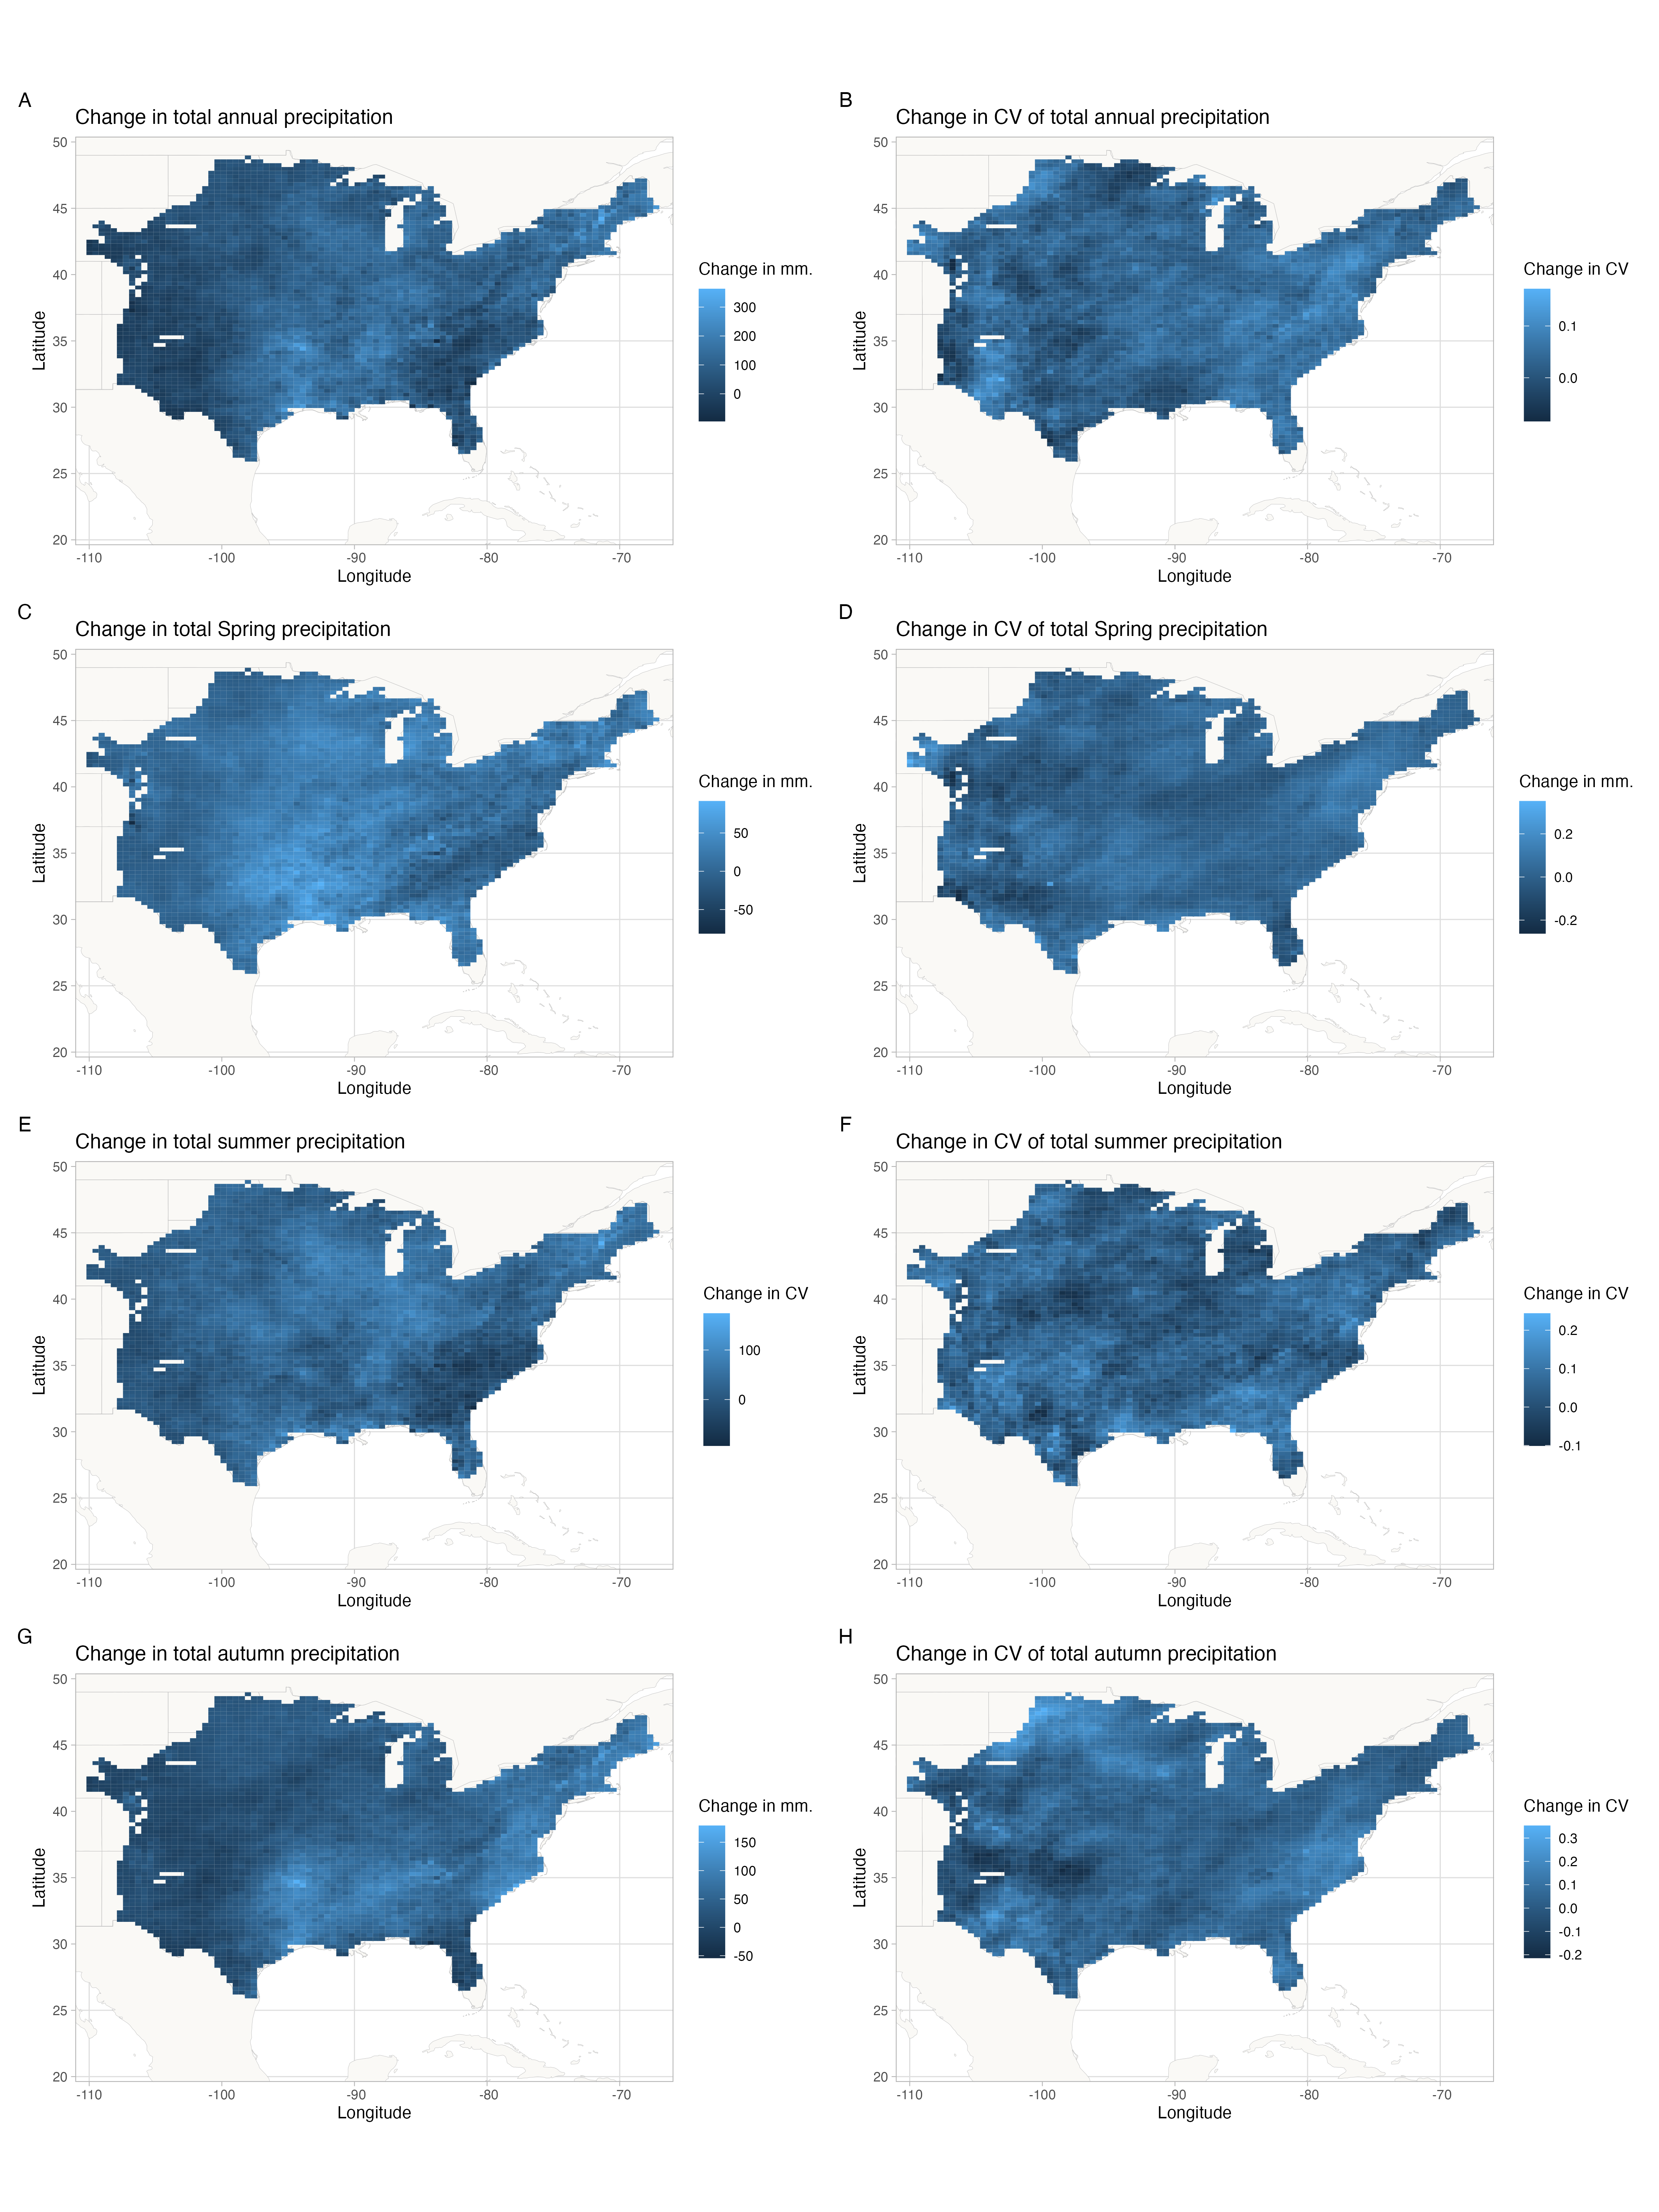
\includegraphics[width = .8\linewidth]{ppt_change_maps.png}
	\caption{\textbf{Change in precipitation between the periods 1895-1925 and 1990-2020.} Color represents change in annual or seasonal total precipitation (A,C,E,G) and in the coeffiecient of variation of annual or seasonal total precipitation (B,D,F,H). Maps show the study area of \emph{A. hyemalis}. Map pixels used in correlation analysis with endophyte change were pulled from studies areas specific to each host species. }
\end{figure}

	
	\begin{figure}[H]
		\centering
		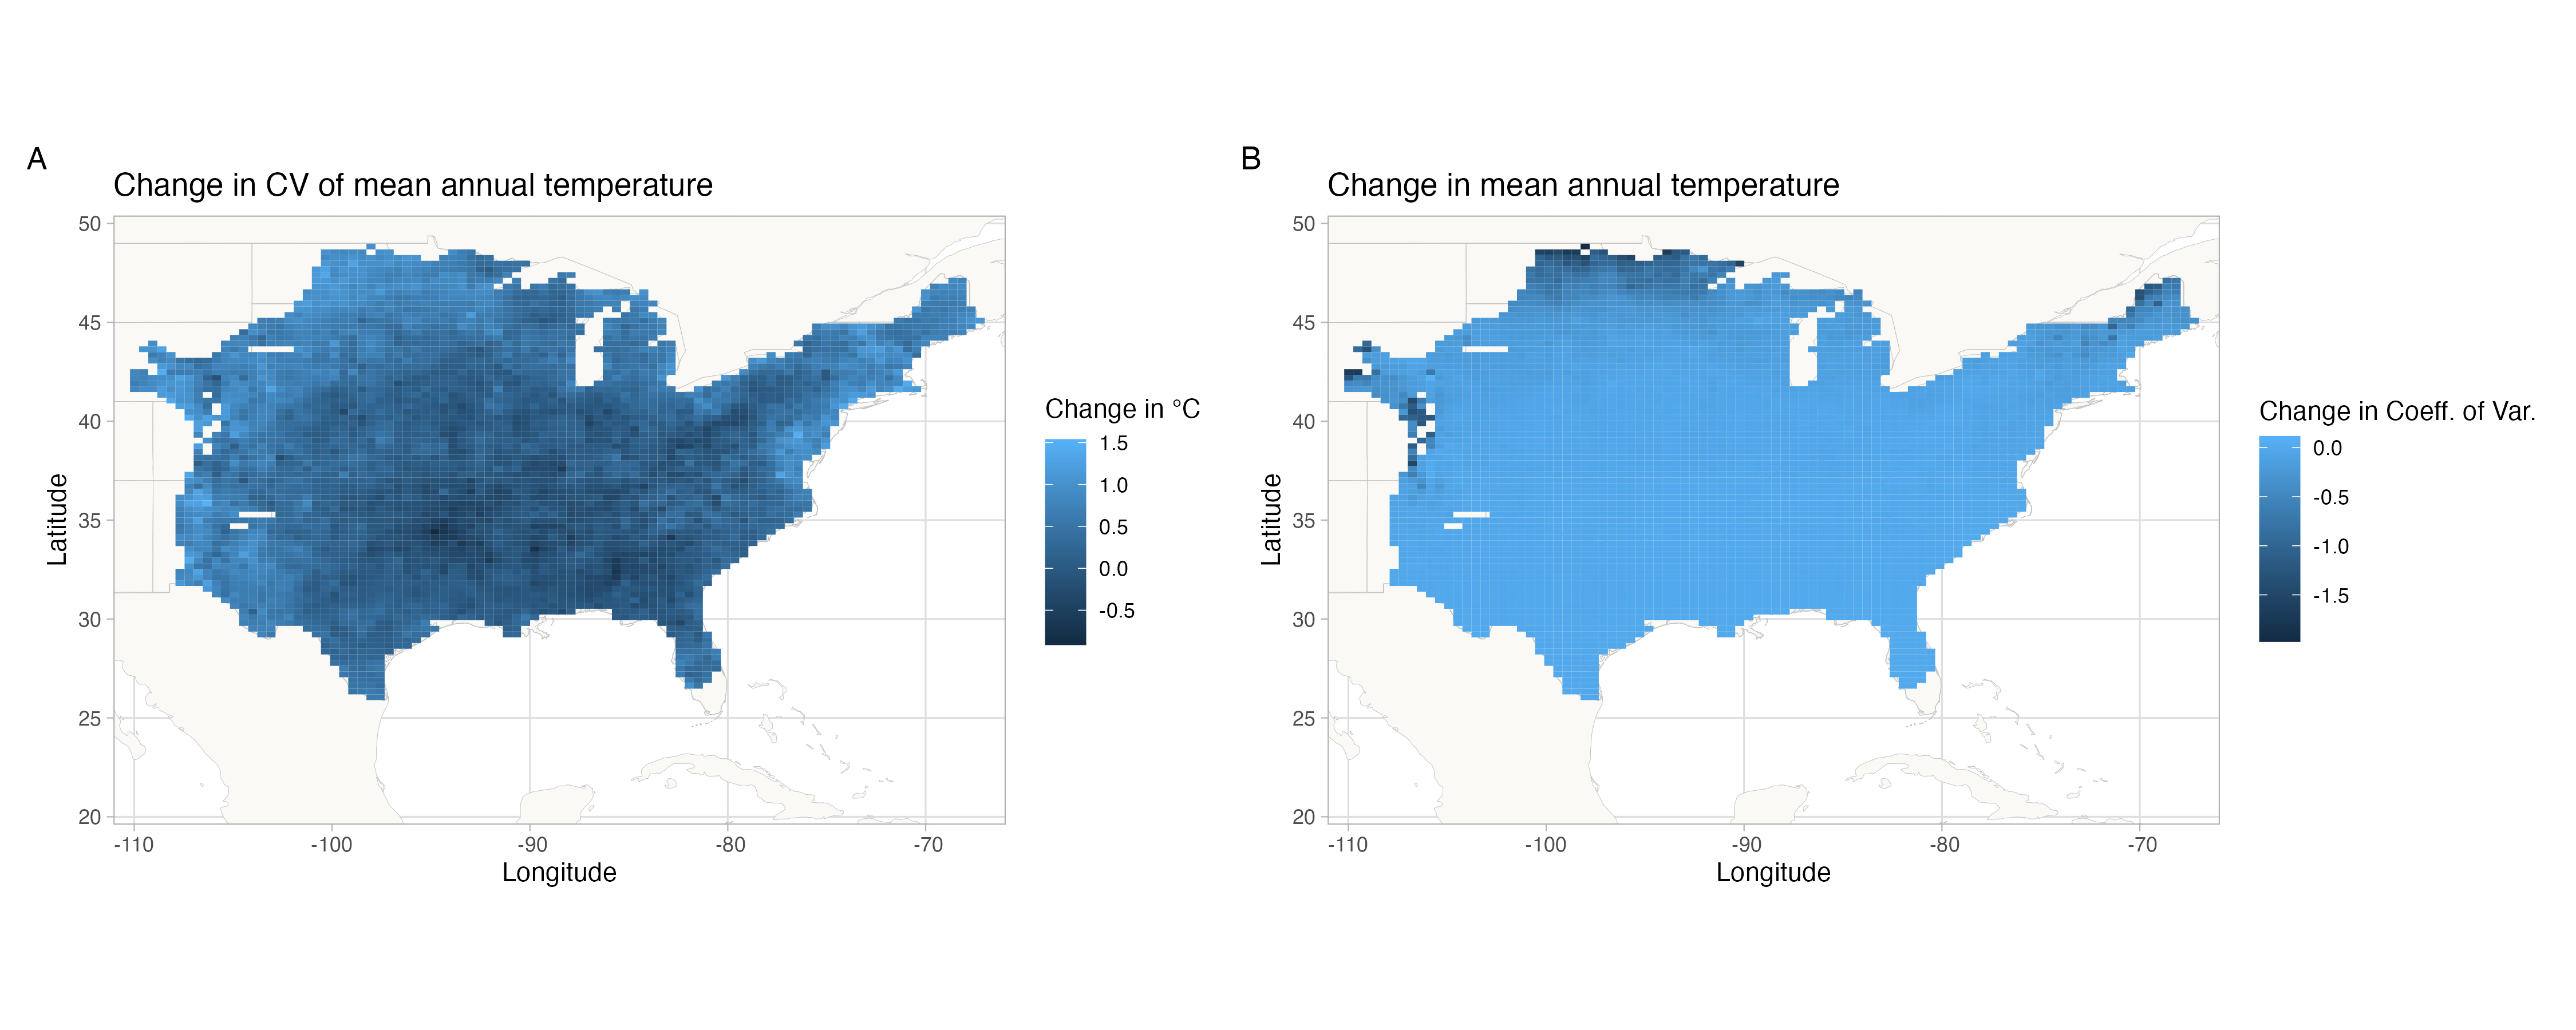
\includegraphics[width = \linewidth]{tmean_change_maps.png}
		\caption{\textbf{Change in temperature between the periods 1895-1925 and 1990-2020.} Color represents change in annual mean temperature (A) and in the coeffiecient of variation of annual mean temperature (B). Maps show the study area of \emph{A. hyemalis}. Map pixels used in correlation analysis with endophyte change were pulled from studies areas specific to each host species.}
	\end{figure}



\begin{figure}[H]
	\centering
	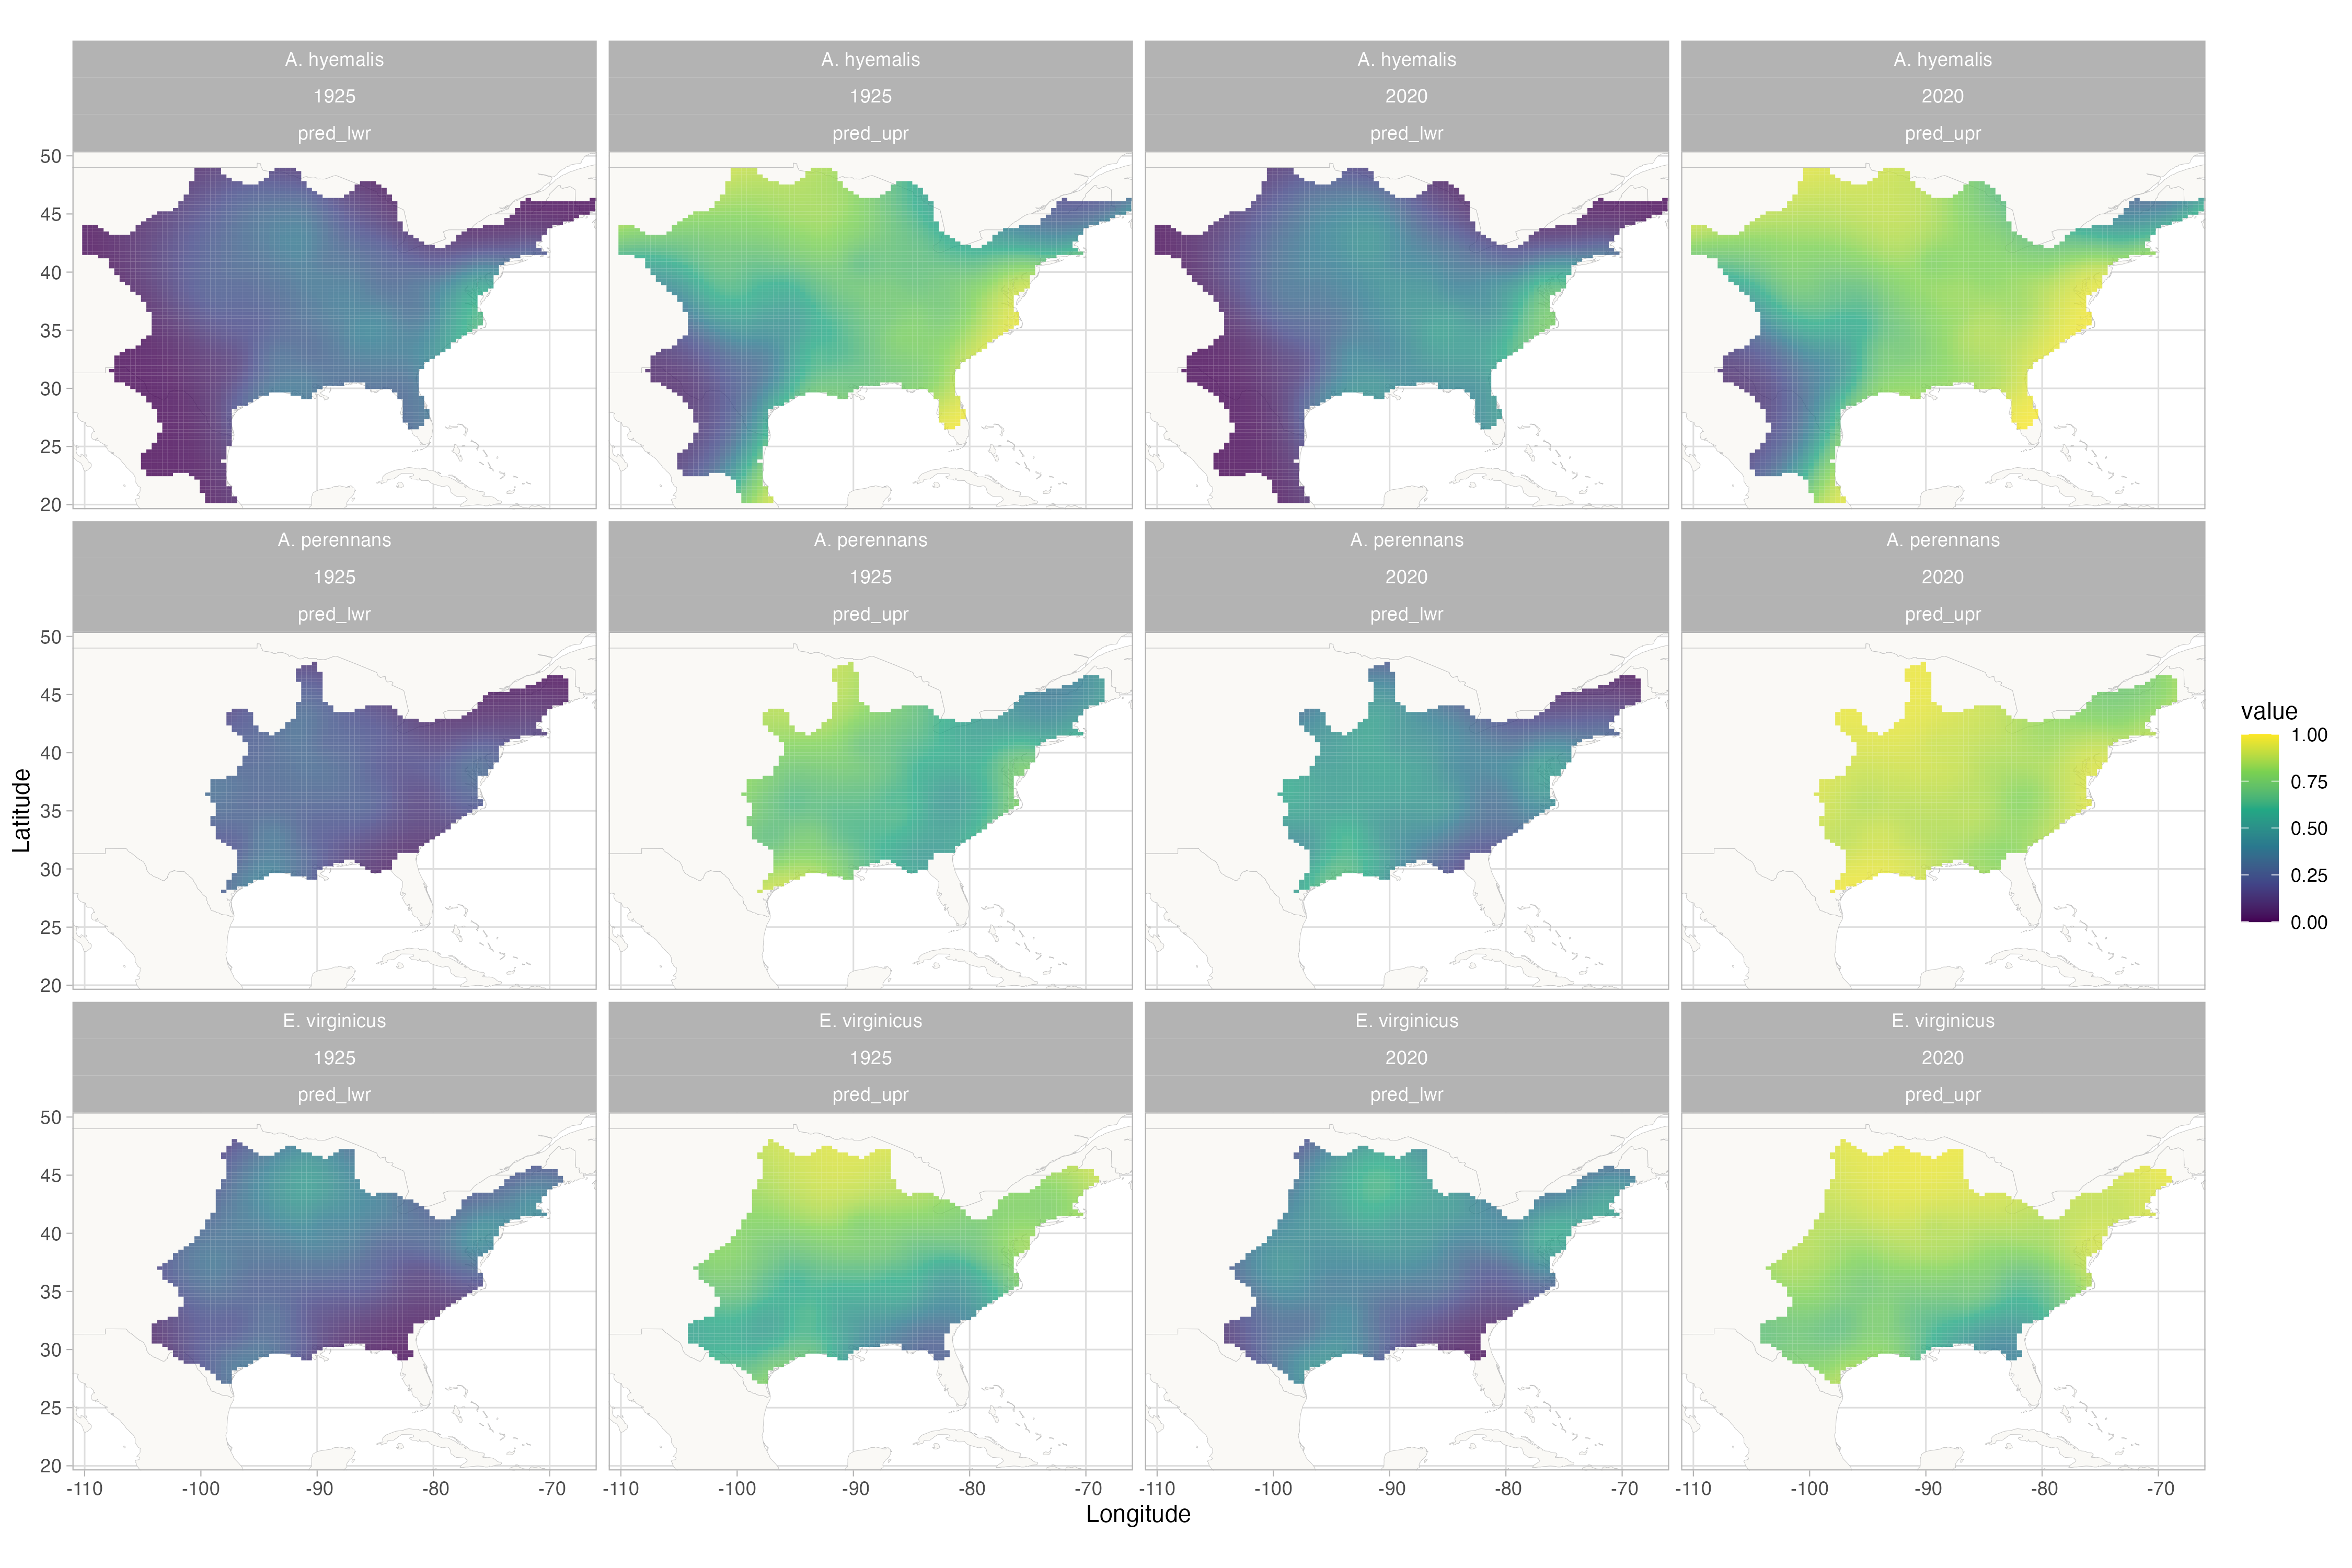
\includegraphics[width = \linewidth]{prevalence_map_CI.png}
	\caption{\textbf{Uncertainty associated with spatial trends in endophyte prevalence.} Color represents change in predicted endophyte prevalence. Panels show upper and lower 95\% posterior probability for each host species between 1925 and 2020.}
\end{figure}


\begin{figure}[H]
	\centering
	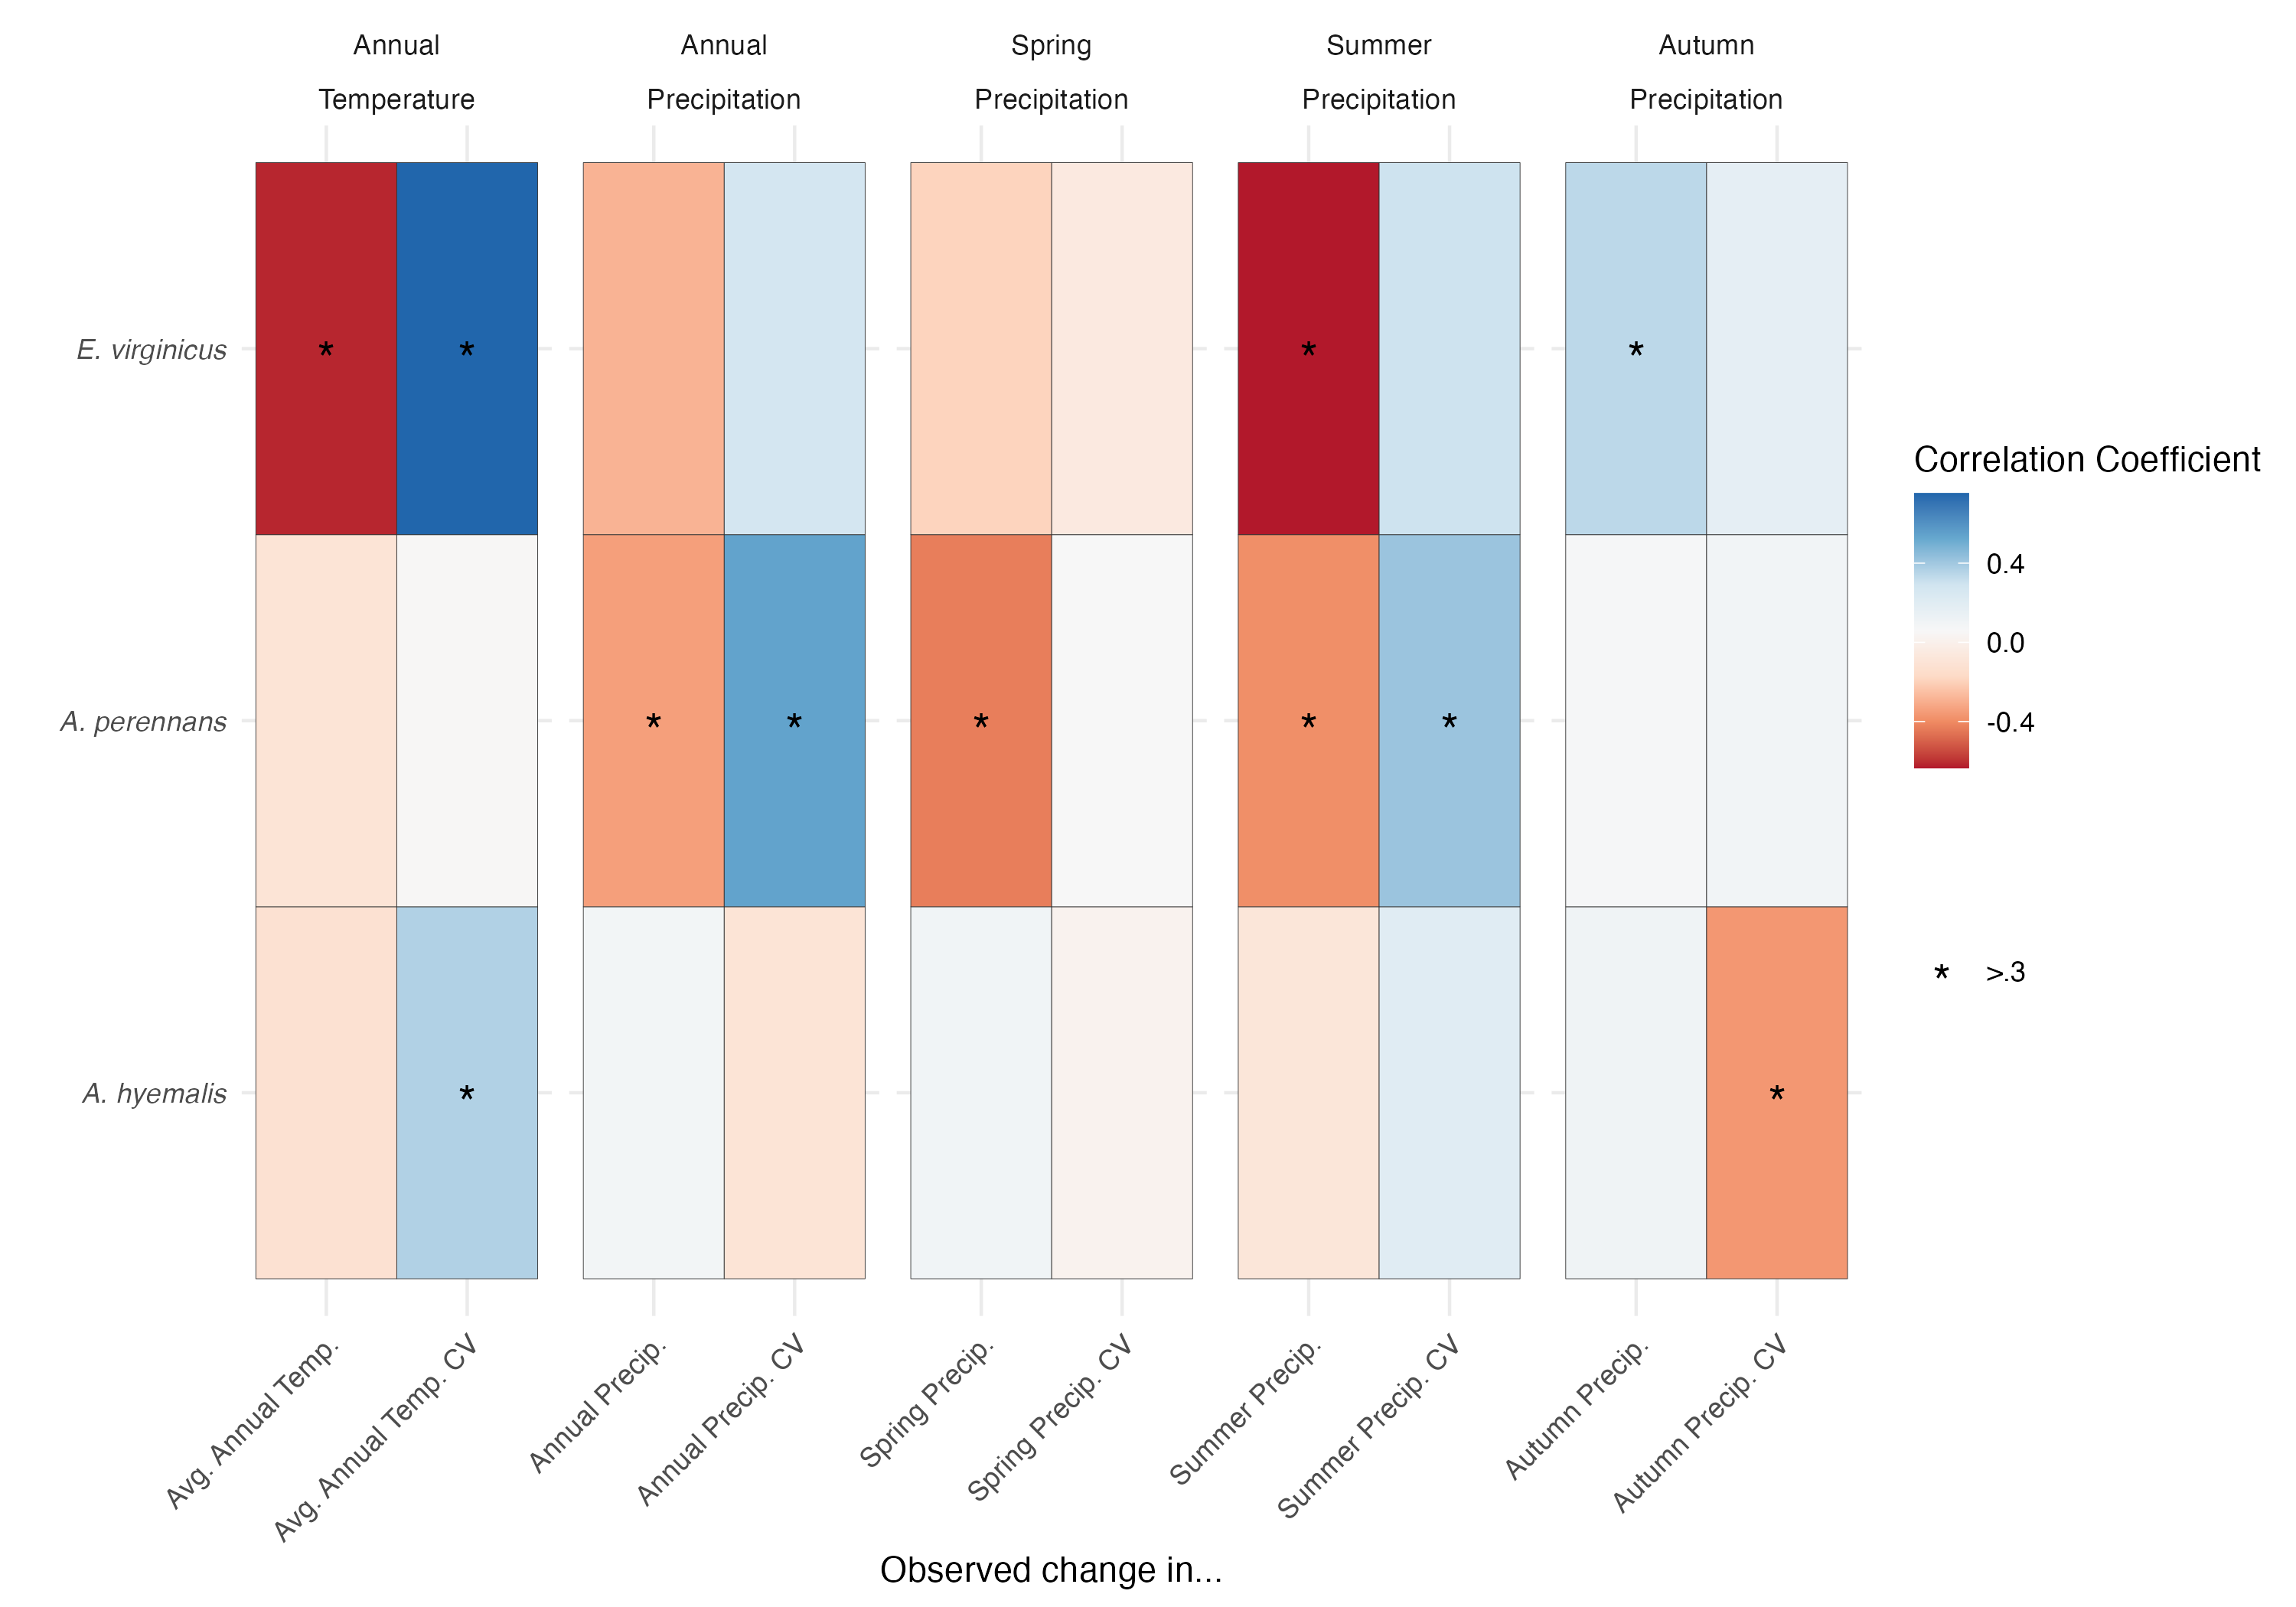
\includegraphics[width = \linewidth]{climate_corr_heatmap_subsample.png}
	\caption{\textbf{Correlations between changes in climate drivers and changes in endophyte prevalence from a random sample of 100 pixels across the study region.} Color denotes the Spearman correlation coefficient between the relative rate of change in endophyte prevalence and the change in annual mean temperature ($^oC$) and total annual and seasonal precipitation (mm), as well as the change in the coefficient of variation of each climate driver. Positive correlation coefficients indicate that greater increases in a climate driver were associated with larger increases in endophyte prevalence, while negative values indicate that . Asteriks denote correlation coefficients $> .3$ or $< -.3$.}
\end{figure}


	
	\begin{table}[h]
		\caption{Summary of herbarium samples across collections}
		\label{Table:herbaria}
		\centering
		\begin{tabular}{llll}\hline
			Herbarium Collection        & AGHY        & AGPE      &      ELVI\\ \hline
			Botanical Research Institute of Texas &   341   &    189&    176    \\
			Louisiana State University &     71  & --  &   61       \\
			Mercer Botanic Garden &   3    & --     &     6\\
			Missouri Botanic Garden& 78 & 39& 31\\
		    Texas A\&M &  73&-- & 49 \\
		    University of Kansas & 134 & -- &  20\\
		    University of Oklahoma & 65 &30&  91\\
		    University of Texas  \& Lundell   &  169& 41& 99\\		    				 			     			     
			Oklahoma State University&     30  &   --    &  69 \\ \hline
		\end{tabular}
		\bigskip{}

	\end{table}
	
	
	
	
	% In most cases, authors should typeset supplementary material in a separate,
	% author-supplied PDF. For author-supplied PDFs, please consult the
	% AmNat_supp_template.tex document, available from
	% https://www.journals.uchicago.edu/journals/an/instruct 
	%
	% By contrast, the Appendix instructions below apply to cases in which
	% a brief appendix is to appear in print after the main body of the article.
	% That notably includes descriptions of methods, tables defining parameters,
	% and other material necessary for reproducing the MS's results.
	%
	% Please reset counters for the appendix (thus normally figure A1, 
	% figure A2, table A1, etc.).
	%
	% Most AmNat articles have no more than one print appendix. If your article
	% has more than one, counters for each appendix should match the letter of
	% that appendix. For example, tables in Appendix B should be numbered table B1, % table C2, etc. This applies to tables, equations, and figures.
	%
	% It's better not to use the \appendix command, because we have some
	% formatting peculiarities that \appendix conflicts with.
	
	%%%%%%%%%%%%%%%%%%%%%
	% Bibliography
	%%%%%%%%%%%%%%%%%%%%%
	% You can either type your references following the examples below, or
	% compile your BiBTeX database and paste the contents of your .bbl file
	% here. The amnatnat.bst style file should work for this---but please
	% let us know if you run into any hitches with it!
	%
	% If you upload a .bib file with your submission, please upload the .bbl
	% file as well; this will be required for typesetting.
	%
	% The list below includes sample journal articles, book chapters, and
	% Dryad references.
	\newpage{}
\bibliographystyle{plainnat}
\bibliography{endo_herbarium}
	
	\newpage{}
	

	
\end{document}

